%%%%% STYLES AND STUFF 
\documentclass[a4paper,oneside,onecolumn,openright,12pt]{book}


\makeatletter

%
\usepackage{caption}
\usepackage{subcaption}
\usepackage{footmisc}
\usepackage{paralist}
\usepackage{amsthm}
\usepackage{subfig}

% Fonts, encoding, etc.
\usepackage{type1cm}
\usepackage[latin1]{inputenc}
\usepackage[british]{babel}
\usepackage[T1]{fontenc}
\usepackage{times}
\usepackage{hyperref}
\usepackage[all]{hypcap}
\usepackage{longtable}
\usepackage{algorithm}
\usepackage{algpseudocode}
\usepackage{multirow}
\usepackage{float}


% Line spacing
\def\baselinestretch{1.5}
\parindent0cm
\parskip1.5ex\@plus.7ex\@minus.1ex\relax

%Acronyms
 \usepackage{acronym}
 %Inline lists
 \usepackage{paralist}

%Glossary
\usepackage[toc]{glossaries}

% Page dimensions
\usepackage{vmargin}
\setpapersize{A4}
\setmarginsrb{40mm}{20mm}{25mm}{30mm}{14.5pt}{8mm}{0pt}{11mm}

% Footer and header
\usepackage{afterpage}
\usepackage{fancyhdr}
\pagestyle{fancy}
\fancyhead{}
\fancyhead[LE,RO]{\thepage}
\fancyhead[LO,RE]{\slshape \leftmark}
\fancyfoot{}
\renewcommand{\chaptermark}[1]{}
\renewcommand{\sectionmark}[1]%
             {\markboth{\thesection\ #1}{\thesection\ #1}}
\renewcommand{\subsectionmark}[1]{}
\fancypagestyle{plain}{%
  \fancyhead{}
  \fancyhead[LE,RO]{\thepage}
  \fancyfoot{}
  \renewcommand{\headrulewidth}{.6pt}
}

% Chapter
\def\@makechapterhead#1{%
  \ \\[-35.5pt]\hbox to \textwidth {%
    \hfill {\vbox{\hbox{\rule[5pt]{140pt}{4pt}}%
        \hbox to 140pt {\hfill\huge\bfseries\slshape \@chapapp\space\thechapter\/}}}}%
  \vskip55\p@%
  {\parindent \z@ \raggedright \normalfont%
    \interlinepenalty\@M%
    \Huge \bfseries #1\par\nobreak%
    \vskip 45\p@%
  }}
\def\@chapter[#1]#2{\ifnum \c@secnumdepth >\m@ne
                       \if@mainmatter
                         \refstepcounter{chapter}%
                         \typeout{\@chapapp\space\thechapter.}%
                         \addcontentsline{toc}{chapter}%
                                   {\protect\numberline{\thechapter}#1}%
                       \else
                         \addcontentsline{toc}{chapter}{#1}%
                       \fi
                    \else
                      \addcontentsline{toc}{chapter}{#1}%
                    \fi
                    \chaptermark{#1}%
                    \addtocontents{lof}{\protect\addvspace{10\p@}}%
                    \addtocontents{lot}{\protect\addvspace{10\p@}}%
                    \addtocontents{loa}{\protect\addvspace{10\p@}}%
                    \if@twocolumn
                      \@topnewpage[\@makechapterhead{#2}]%
                    \else
                      \@makechapterhead{#2}%
                      \@afterheading
                    \fi}
\def\@schapter#1{\addcontentsline{toc}{chapter}{#1}%
                 \markboth{#1}{#1}%
                 \addtocontents{lof}{\protect\addvspace{10\p@}}%
                 \addtocontents{lot}{\protect\addvspace{10\p@}}%
                 \addtocontents{loa}{\protect\addvspace{10\p@}}%
                 \if@twocolumn%
                    \@topnewpage[\@makeschapterhead{#1}]%
                 \else%
                    \@makeschapterhead{#1}%
                    \@afterheading%
                 \fi}
\def\@makeschapterhead#1{%
  \ \\[-35.5pt]\hbox to \textwidth {%
    \hfill {\vbox{\hbox{\rule[5pt]{140pt}{0pt}\rule[5pt]{0pt}{4pt}}%
        \hbox to 140pt {\hfill\huge\bfseries\slshape \ \/}}}}%
  \vskip55\p@%
  {\parindent \z@ \raggedright \normalfont%
    \interlinepenalty\@M%
    \Huge \bfseries  #1\par\nobreak%
    \vskip 45\p@%
  }}

% Table of contents
\def\contentsname{Contents}
\renewcommand\tableofcontents{%
    \if@twocolumn%
      \@restonecoltrue\onecolumn%
    \else%
      \@restonecolfalse%
    \fi%
    \chapter*{\contentsname}%
    \@starttoc{toc}%
    \if@restonecol\twocolumn\fi%
    }

% Bibliography
\renewenvironment{thebibliography}[1]
     {\chapter*{\bibname}%
      \list{\@biblabel{\@arabic\c@enumiv}}%
           {\settowidth\labelwidth{\@biblabel{#1}}%
            \leftmargin\labelwidth
            \advance\leftmargin\labelsep
            \@openbib@code
            \usecounter{enumiv}%
            \let\p@enumiv\@empty
            \renewcommand\theenumiv{\@arabic\c@enumiv}}%
      \sloppy
      \clubpenalty4000
      \@clubpenalty \clubpenalty
      \widowpenalty4000%
      \sfcode`\.\@m}
     {\def\@noitemerr
       {\@latex@warning{Empty `thebibliography' environment}}%
      \endlist}

% Floats
\long\def\@makecaption#1#2{%
  \vskip\abovecaptionskip
  \sbox\@tempboxa{\textbf{#1: #2}}%
  \ifdim \wd\@tempboxa >\hsize
    \textbf{#1: #2.}\par
  \else
    \global \@minipagefalse
    \hb@xt@\hsize{\hfil\box\@tempboxa\hfil}%
  \fi
  \vskip\belowcaptionskip}
\renewcommand{\topfraction}{0.9}
\renewcommand{\textfraction}{0.1}
\renewcommand{\floatpagefraction}{0.9}

% Tables
\usepackage{dcolumn}
\usepackage{hhline}

% Graphics
\usepackage[dvips]{graphicx}
\usepackage[usenames,dvipsnames]{color}
\usepackage{rotating}
\usepackage{psfrag}
\usepackage{epic}
\usepackage{eepic}


% List of figures and tables
\renewcommand\listoffigures{%
    \if@twocolumn
      \@restonecoltrue\onecolumn
    \else
      \@restonecolfalse
    \fi
    \chapter*{\listfigurename}%
      \@mkboth{\listfigurename}{\listfigurename}%
    \@starttoc{lof}%
    \if@restonecol\twocolumn\fi
    }
\renewcommand\listoftables{%
    \if@twocolumn
      \@restonecoltrue\onecolumn
    \else
      \@restonecolfalse
    \fi
    \chapter*{\listtablename}%
      \@mkboth{\listtablename}{\listtablename}%
    \@starttoc{lot}%
    \if@restonecol\twocolumn\fi
    }

% Math symbols, fonts, etc.
\usepackage{amsmath}
\usepackage{amsfonts}
\usepackage{amssymb}

\newcommand{\N}{\mathbb{N}}
\newcommand{\Z}{\mathbb{Z}}
\newcommand{\Q}{\mathbb{Q}}
\newcommand{\R}{\mathbb{R}}
\newcommand{\C}{\mathbb{C}}
\renewcommand{\S}{\mathbb{S}}
\renewcommand{\P}{\mathbb{P}}
\newcommand{\E}{\mathbb{E}}

\newcommand{\Cf}{\mathfrak{C}}
\newcommand{\Pf}{\mathfrak{P}}

\DeclareMathOperator{\sign}{sign}
\DeclareMathOperator{\avg}{avg}
\DeclareMathOperator{\floor}{floor}
\DeclareMathOperator{\ceil}{ceil}
\DeclareMathOperator{\round}{round}

\providecommand{\abs}[1]{\lvert#1\rvert}
\providecommand{\absd}[1]{\left\lvert#1\right\rvert}
\providecommand{\card}[1]{\lvert#1\rvert}
\providecommand{\norm}[1]{\lVert#1\rVert}

% URLs
\usepackage{url}
%% Define a new 'leo' style for the package that will use a smaller font.
\makeatletter
\def\url@leostyle{%
  \@ifundefined{selectfont}{\def\UrlFont{\sf}}{\def\UrlFont{\footnotesize\ttfamily}}}
\makeatother
%% Now actually use the newly defined style.
\urlstyle{leo}




% STUFF I ADDED:

\usepackage{thmbox}
\newtheorem[S,leftmargin=18pt,thickness=0.9pt,bodystyle=\noindent]{mydefinition}{Definition}[chapter]
\newtheorem[S,leftmargin=18pt,thickness=0.9pt,bodystyle=\noindent]{myproposition}{Proposition}[chapter]
\newtheorem[S,leftmargin=18pt,thickness=0.9pt,bodystyle=\noindent]{myobservation}{Observation}[chapter]

\usepackage{amssymb}
\usepackage{graphicx}
\usepackage{float}
\usepackage{pgfplots}
\usepackage{pgfplotstable}
\pgfplotsset{
    % #1: index in the group(0,1,2,...)
    % #2: number of plots of that group
    bar group size/.style 2 args={
        /pgf/bar shift={%
                % total width = n*w + (n-1)*skip
                % -> subtract half for centering
                -0.5*(#2*\pgfplotbarwidth + (#2-1)*\pgfkeysvalueof{/pgfplots/bar group skip})  + 
                % the '0.5*w' is for centering
                (.5+#1)*\pgfplotbarwidth + #1*\pgfkeysvalueof{/pgfplots/bar group skip}},%
    },
    bar group skip/.initial=2pt,
    plot 0/.style={blue,fill=blue!30!white,mark=none},%
    plot 1/.style={red,fill=red!30!white,mark=none},%
    plot 2/.style={brown!60!black,fill=brown!30!white,mark=none},%
}

\usepackage{listings}
\usepackage{color}
\lstset{ %
  language=Octave,                % the language of the code
  basicstyle=\footnotesize\ttfamily,           % the size of the fonts that are used for the code
  numbers=left,                   % where to put the line-numbers
  numberstyle=\tiny\color{black},  % the style that is used for the line-numbers
  stepnumber=2,                   % the step between two line-numbers. If it's 1, each line 
                                  % will be numbered
  numbersep=5pt,                  % how far the line-numbers are from the code
  backgroundcolor=\color{white},      % choose the background color. You must add \usepackage{color}
  showspaces=false,               % show spaces adding particular underscores
  showstringspaces=false,         % underline spaces within strings
  showtabs=false,                 % show tabs within strings adding particular underscores
  rulecolor=\color{black},        % if not set, the frame-color may be changed on line-breaks within not-black text (e.g. commens (green here))
  tabsize=3,                      % sets default tabsize to 3 spaces
  captionpos=b,                   % sets the caption-position to bottom
  breaklines=true,                % sets automatic line breaking
  breakatwhitespace=false,        % sets if automatic breaks should only happen at whitespace
                                  % also try caption instead of title
  keywordstyle=\color{blue},          % keyword style
  commentstyle=\color{dkgreen},       % comment style
  stringstyle=\color{mauve}      % string literal style
}


% FUNCTIONS:

% retweet group
\newcommand{\rg}[1]{RG(#1)}

% retweets 
\newcommand{\rt}[1]{RT(#1)}

% retweet count
\newcommand{\rc}[1]{#1.\textrm{count}_R}

% expected retweet count
\newcommand{\ec}[1]{e(#1)}
\newcommand{\ecg}[1]{e_G(#1)}
\newcommand{\ecu}[1]{e_U(#1)}

% follower count
\newcommand{\foc}[1]{\textrm{deg}^+(#1)}

% friend count
\newcommand{\frc}[1]{\textrm{deg}^-(#1)}

% author
\newcommand{\aut}[2]{#1.\textrm{author}_#2}

% set of followers
\newcommand{\fos}[1]{N^+(#1)}

% set of friends
\newcommand{\frs}[1]{N^-(#1)}

% raw audience
\newcommand{\raa}[1]{\textrm{audience}(#1)}

% distinct audience
\newcommand{\dia}[1]{\textrm{audience}(#1)}

% interestingness score
\newcommand{\score}[1]{s(#1)}
\newcommand{\gscore}[1]{s_G(#1)}
\newcommand{\uscore}[1]{s_U(#1)}
\newcommand{\ascore}[1]{s_{\textrm{avg}}(#1)}

% score disparity
\newcommand{\disparity}[1]{d(#1)}
\newcommand{\gdisparity}[1]{d_G(#1)}
\newcommand{\udisparity}[1]{d_U(#1)}
\newcommand{\sdisparity}[1]{d_{\textrm{sel}}(#1)} % disparity between SELECTED tweets in question #1

% END OF STUFF I ADDED

\makeatother


\begin{document}


%%%%% FRONT STUFF	
\frontmatter

\begin{titlepage}

\begin{center}
\vspace*{3ex}
\textbf{\Huge The Detection and Inference of  the Interestingness of Information in Online Social Networks}\\[2ex]

\textbf{\LARGE Will Webberley}\\
\vfill
\textbf{\LARGE 2013}\\
\vfill
\textbf{\LARGE Cardiff University}\\[1ex]
\textbf{\LARGE School of Computer Science \& Informatics}\\[4ex]
\end{center}

\end{titlepage}

\chapter*{Abstract}
Abstract text here etc.

\tableofcontents
\listoffigures
\listoftables
\chapter*{List of Acronyms} 
\begin{acronym}
% to use in the thesis, use: \ac{OSN}
\acro{OSN}{Online Social Network}
\acro{MTW}{Mechanical Turk Worker}
\acro{URL}{Uniform Resource Locator}

\end{acronym}

\chapter*{Glossary} 

{\bf Follower}
A type of user. A user, \textit{x}, is a follower of user \textit{y} if user \textit{x} follows user \textit{y}. Other users who follow a particular user will receive all of the user's Tweets and retweets to their home timeline. A user can elect to follow another user.

{\bf Friend}
The inverse of follower. User \textit{x} is a friend to user \textit{y} if \textit{y} follows \textit{x}.

{\bf Path-length}
The penetration of a Tweet - i.e. the number of times a Tweet is retweeted down one chain. The final retweeter in the chain indicates the number of hops the Tweet has taken from its author.
			
{\bf Retweet}
\textit{n.} - A replica of a Tweet, which has been forwarded on by a user (who is not the Tweet's original author) to their own followers. \\
\textit{v.} - The act of replicating a Tweet. A user who finds a Tweet interesting may retweet it so that it gets more exposure.
									
{\bf Retweet Group}
Set of Twitter users responsible for the propagation of a Tweet. Comprises the original author of the Tweet and the users which have since retweeted it.

{\bf Retweet Count}
The number of times a particular Tweet has been retweeted.

{\bf Timeline}
A collection of Tweets in Twitter in reverse-chronological order. A user timeline consists of that user's Tweets. A user's home timeline consists of the Tweets of each friend of the user.

{\bf Tweet}
\textit{n.} - A piece of information in Twitter; a piece of text, less than 240 characters long, which is written by a user. When sent, the Tweet is sent to the home timelines of each of the followers of the Tweet's author.\\
\textit{v.} - The act of writing and sending a Tweet.

{\bf User}
An account on Twitter. Each user (usually representing a real-life person or organisation) can Tweet, retweet, follow other users and be followed by other users. In this thesis, sometimes the terms \textit{user} and \textit{person} are used interchangeably.


%%%%% MAIN STUFF 
\mainmatter 

\chapter{Introduction}
\chapter{Introduction}

Online social networks have exploded into the lives of millions of people worldwide over the last decade, and their use has dominated the communication highways and facilitated the interconnection of the world in ways never before perceived possible.

These social networks imitate real-world social networks. Although most such platforms each provide a different service to collaboratively satisfy an array of different use-cases, they tend to all be based around the idea of `friendships' (i.e. links between the user nodes in the social graph) and the sharing of information amongst friends.

Social networks like these have been available for around ten years now (with MySpace\footnote{http://myspace.com} launching in 2003 and Bebo\footnote{http://bebo.com} in 2005), but it wasn't really until Facebook's\footnote{http://facebook.com} worldwide launch in 2006 that social networks became the staple, ubiquitous norm that they are today. More recently, we have seen the introductions of Google's social network grown from its Buzz service, Google Plus\footnote{http://plus.google.com}, Pinterest\footnote{http://pinterest.com}, App.net\footnote{http://app.net}, and many more. They make up a large part of the basis and meaning behind the ideas of Web 2.0, which describes the web as being primarily formed from user-generated content and encourages the sharing of such content.

Another component that helped in the dawn of Web 2.0 was the rise of \textit{blogging}. A blog (`web-log') is a time-based series of posts consisting of continuous pieces of text, photos, or other media, and is generally contributed to by a single author. Blogs are often based around one or a set of topics and are usually public - meaning that they are written with the intention of being read by others. Despite this, they are often a way in which the author can look back at their history of posts, acting more as a diary recording snapshots of the author's life.\\
Various blogging services exist on the web today, such as Medium\footnote{http://medium.com}, Wordpress\footnote{http://wordpress.com}, and Tumblr\footnote{http://tumblr.com}.


\section{Twitter as a Social Network}
Twitter\footnote{http://twitter.com} is an online social network, which launched in the summer of 2006 \cite{krishnamurthy08}. Since then, it has rapidly gained in popularity amongst several different user groups - teens and young people, casual users, celebrities, reporters, and so on - and within eight months had around 94,000 registered users \cite{java07}. Although Twitter has never been a direct competitor with Facebook, users tend to use the two sites concurrently for different purposes: whilst Facebook's focus is on providing many services at once (such as photo-sharing, commenting/endorsing of information, messaging, pages for businesses, groups, events, etc.), Twitter's is more on simplicity.

More specifically than just being an online social network, Twitter is a microblogging website. Whilst a blog, as mentioned, typically contains long posts, Twitter only allows its users to post short pieces of text, up to 140 characters in length \cite{krishnamurthy08} \cite{huberman08}, called `Tweets'. Thus, Twitter is a hybrid social network and blogging service and whilst each Tweet may only realistically be able to hold a couple of sentences, this system facilitates quick, timely, and `real-time' \textit{live} information-sharing amongst its millions of users \cite{zhao09}. Its idea is that short pieces of news will `travel' faster and will be seen by more people more quickly than traditional news stories.

Although Tweets are limited to 140 characters in length, the inclusion of URLs is allowed. This enables further extension of Tweets through external websites, and supports the inclusion of links to images and videos. Twitter has encouraged this use-case by providing `share' buttons for developers to embed in websites, and direct support for photo and video applications, such as TwitPic\footnote{http://twitpic.com} and Vine\footnote{http://vine.com}.

Its simplicity has also helped its growth into the mobile domain, in which smartphone users are able to very quickly post updates about their lives, a piece of information they want to share, or a photo or video, and be able to post it \textit{as it happens} directly from the news source or geographical location \cite{castillo11}. This has been especially useful in emergency situations worldwide, including the Haiti earthquake in 2010 \cite{muralidharan11}, and 2011's Egyptian protests \cite{wilson11} and Thai flood \cite{kongthon12}.\\
Indeed, \cite{sakaki10} used Twitter to build an earthquake-reporting system for Japan that outperforms the Japan Meteorological Agency in terms of its promptness of notification.

Use of Twitter is based around `timelines' of Tweets, to which new Tweets are pre-pended as they are posted by users. The \textit{home} timeline is the default view, in which Tweets from all of a person's subscribed-to users are placed. Timelines of an individual user contain only Tweets from that user, and are known as a `user' timeline. Customisation of timelines is also possible through the use of Twitter lists, in which different users can be placed to categorise streams of Tweets from different sets of users.


\section{Twitter's Social Graph and Information Subscription}
As with many social networks, the structure of Twitter lies within the users and their connectivity within its social graph. However, unlike Facebook, whose social structure is made up of bi-directional `friendships' between users, Twitter's primary social graph is made up more of mono-directional links between its users \cite{edwards13}. A person using Twitter can elect to \textit{follow} another user, which subscribes the person to receive all of that user's Tweets to their home timeline. The set of users that follow a person are known as that person's \textit{followers}, and the set of users that the person follows are the person's \textit{friends}.\\
Therefore, if two users both mutually follow each other, then the link between them is bi-directional.

Whilst bi-directional links are common amongst communities of similar interests, friends, colleagues, and so on, mono-directional links are found more in situations in which less-influential users follow more-influential users, such as celebrities.


\section{The Problem}
A user who follows a set of other users can \textit{generally} be said to find that set of users to produce more interesting information than those users that the user does not follow. However, despite that, not \textit{all} information produced by an `interesting' user is likely to be interesting, and yet \textit{all} information produced by a Twitter friend will be received onto the home timeline.\\
Noise is a common problem in Twitter, and is the uninteresting information one might receive that conveys little interest. It is likely that most of the information received on Twitter \textit{is} uninteresting \cite{alonso10}, and this makes it very hard to distinguish the interesting information from the uninteresting.

Since people tend to use Twitter most in short sporadic moments, looking for a quick news fix, they do not have time to filter out noisy information. Thus, the presence of noise can dampen the experience of the user, making it much more difficult to find interesting information.

In addition, Twitter users typically exist within an information `bubble'. This is similar to the notion of the Google search bubble, in which the search engine uses previous results and search terms to only return information to a user based on what \textit{it thinks} the user would find the most interesting and useful.\\
This results in the users not knowing which information exists beyond the confines of their bubble, and if they do not know it exists, they cannot know if it is of interest to them. Similarly, a Twitter user cannot follow all of the users he/she may find interesting, since he/she will not \textit{know} of all the interesting users existing on the social graph.

How can users be exposed to \textit{interesting} and \textit{relevant} information, but without them having to know about it or look for it first?


\section{Contributions}
This thesis focuses on understanding information propagation, and how this combined with knowledge of the social structure of Twitter can assist towards solving the problem of identifying interesting and relevant information and determining it from the noise on Twitter. 
Whilst other work in the area has also looked into the notions of relevance and interest in online social networks, and Twitter in particular, none has addressed the problem in such a way as this.

Part of the outcome of this research are methods for effectively inferring interesting information and, indeed, ranking information by interestingness. The methods are validated in various ways to help highlight their strengths and weaknesses in performing inferences and appropriate use-cases.

The work addresses the problem area in that it helps towards solving the goal of identifying \textit{globally} interesting information in Twitter. In addition, certain measures are taken in an attempt to address the idea of information relevance, which denotes how information interestingness is subjective, and thus different from user to user.


\section{Thesis Structure}
The rest of this thesis is structured as follows.

A background is provided as an introduction to some of the ideas behind the main research, which immediately follows this chapter, and includes a review of relevant literature across the range of topics addressed in the thesis.\\
Following this are chapters that contain research on Twitter's information propagation characteristics and its interesting and useful behaviours, the social structure of Twitter and the ways in which this is important for understanding the spread of information, and then on the research of the methodologies themselves, including validation and analysis of the results of this work.

The thesis ends with a general analysis and conclusion, and a discussion of potential future work in this area and leading on from this research.

\chapter{Background}
\chapter{Background}


One of the most widely-used features of Twitter is its inbuilt function for facilitating the spread of information within its social structure. This phenomenon is the basis for much of the research in this thesis and, when combined with the characteristics of Twitter's user graph, has many interesting attributes and behaviours associated with it.


\section{Domain Context}

\subsection{Information Propagation through Retweeting}
The function of propagation in Twitter is known as \textit{retweeting}, and is carried out by the Twitter users themselves. When a user views a Tweet that they believe to be particularly interesting, and believe it to also be interesting to his/her followers, then he/she can elect to retweet it, and thus pass it further through the social graph to that user's followers also. A Tweet that has been retweeted is known as a \textit{retweet}, and it is clear that a Tweet which is retweeted will be made available to significantly more users than a Tweet that isn't retweeted \cite{webberley11} \cite{kwak10}.

Since Twitter's social graph is decentralised and retweeting occurs between individual groups of users, its properties are similar to information dissemination in other types of decentralised graphs, such as content-forwarding in opportunistic networking \cite{allen10}.

A retweet can be carried out in one of two ways: either through the use of Twitter's native retweet button, or manually. \\
The retweet button is displayed along with each Tweet in a Tweet timeline which, when clicked, immediately creates a new retweet containing the verbatim content of the original Tweet and automatically sends it on to the retweeter's followers.\\ The user who created the original Tweet is credited as the author on the recipients' timelines, with an indication of who carried out the retweet itself. Thus, users who follow the retweeter will see a Tweet appear in their home timeline from someone that they may not directly follow.\\

\begin{figure}[h]
\centering

\includegraphics[scale=0.3]{2.Background/Media/northern_lights_tweet.png} 
\caption{A retweeted Tweet}
\label{fig:northern_lights_tweet}
\end{figure}

The manual approach involves physically copying the content of the Tweet to be retweeted and pasting it into a new Tweet, usually with the text `\texttt{RT @<username>:}' pre-pended, where \texttt{RT} stands for \textbf{r}e\textbf{t}weet and \texttt{<username>} is the username of the author of the original Tweet. This method allows for annotating the original content of the Tweet (for example, to provide an opinion on the Tweet contents), producing a \textit{modified} Tweet, which can sometimes be pre-pended with \texttt{MT} rather than \texttt{RT}.

\begin{figure}[h]
\centering

\includegraphics[scale=0.3]{2.Background/Media/retweet_button.png} 
\caption{The retweet `button' in context}
\label{fig:retweet_button}
\end{figure}

Each Tweet has a retweet count associated with it, which is the raw representation of the number of times that the Tweet has been retweeted using the retweet button method.\\
Since the manual retweet technique is more community-driven, there is no official way to include these as part of the retweet count of the original Tweet. However, since the manual method is typically only really used with the aim to annotate or modify the Tweet in some way, the resultant `retweet'  is no longer a real representation of the content of the original Tweet anyway, and so should not be counted as such.

It should be noted that Twitter users may choose to make their account `protected'. A person who has a protected account will still have a publicly-visible profile (displaying a name, username, bio, and so on), but their Tweets and other information (such as the followers and friends lists) are hidden from users that aren't followers of the person. Potential followers of a protected account must \textit{request} a followship, which can then be accepted or rejected by the protected account holder. \\
Since Tweets from a protected account are only visible to approved followers, the retweet button is unavailable for them to disseminate the Tweet any further than the author's immediate local follower network. However, since the manual retweet method does not rely on the button and isn't governed by Twitter, a protected account's Tweets can still be retweeted in this way.

In a similar way to Facebook supporting the endorsement of information found on its site by inviting users to `like' a piece of content, retweeting is effectively a \textit{vote} or endorsement for a Tweet on Twitter. In both cases, the number of likes and number of retweets is visible to the platforms' respective users, and so this provides some insight into the \textit{popularity} of the information.\\


\subsection{Retweets and the Social Graph}
The social graph of Twitter is constructed, like in other online social networks, by edges between users, partially emulating real-life social interactions between humans. The growth of social media has encouraged more dense communication between users all over the world, who would not previously be able to be in direct contact with one another in this way.

Derived from this, Stanley Milgram's finding of ``six degrees of separation'' \cite{milgram67}, which defines that people are usually no more than six hops away from each other on the `real-life' social graph, was found to be an overestimate when it comes to the analysis of the structure of OSNs by \cite{backstrom11}, who found that the average `distance' observed in Facebook's entire 721 million-node graph in 2011 was only around 4.7 hops. This implies that denser links between users and larger communities that apparently manifest themselves in OSNs create a smaller `world' than that experienced in reality.

In each of Milgram's experiments participants passed a message to one another, at each stage only passing to other people that they actually \textit{know}, in the hope of the it reaching a single intended recipient. This meant that people could use acquaintances in other geographic locations to transfer the message from community to community.\\
Twitter supports a similar propagation mechanism in the fact that retweets can themselves be retweeted; this is a focus of some of the earlier research in this thesis.

This behaviour provides further penetrative `depth' of the information through the social network away from the source user in addition to the spread `width' made by the initial retweets. Although retweeting is not carried out with the aim of information reaching any particular final user (or set of), as with Milgram's experiment, this phenomenon allows retweets to `travel' between `online communities' of users.

As with real-life social networks, communities of users in OSNs are also a common feature \cite{ugander11}.\\
In Twitter, these communities are typically small to begin with and are based on a topic of interest or around a more influential user. As more Tweets are produced from within the community, further links are made to interconnect the community's users, producing a growing `swarm' of interest around the initial topic or user \cite{java07}. \\
As further users begin associating themselves with this community, its audience becomes more widespread and the community grows. This concept is discussed in greater length by \cite{java07}, who also experiment further with communities and describe them as compact groups of users connected by dense follower links.

\begin{figure}[h]
\centering
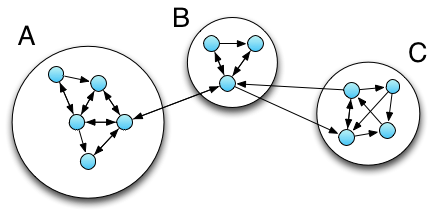
\includegraphics[scale=0.7]{2.Background/Media/communities.png} 
\caption{A hypothetical group of user communities}
\label{fig:communities}
\end{figure}

In more dense communities, Tweets can be made available to many users immediately after they are published, since many of the links between users are shared. This means that any retweets that occur within communities are likely to have a lot of \textit{redundancy}, in that many of the retweets will be sent to users who have already seen the Tweet. Although Twitter prevents this information duplication by not showing the retweets of Tweets that have already appeared on a user's timeline, it does increase the chance of the Tweet making its way out of the community.

Retweets amongst users within a community are likely to be common, due to the shared-interest nature of communities, and some users can provide `bridges' by being active in more than one community. In these cases, Tweets can be passed between the communities through retweets by the bridging user. If there are many users sharing communities, then there are many more avenues available for propagation to occur down, causing a high level of information throughput. If there are fewer bridges, then there is more of a bottleneck between the communities, hindering the information spread.

\cite{java07} also finds that communities can be formed from different types of people, such as those who Tweet frequently and have many followers, and those who contribute very little and have few followers. Those with many followers and many friends receive lots of information and have the potential to spread information further than those with fewer inward and outward edges. Studies in the behaviour of different types of users in Twitter is done more thoroughly in \cite{krishnamurthy08}, which defines `broadcasters' (users with many followers and few friends) and `miscreants' (users with few followers but many friends) and their roles in information propagation.

Users that retweet the interesting information from a source user to others, who do not follow the source user and so would not naturally receive the information, are effectively acting as information \textit{filters}. By not following the source user, a person might still receive the interesting information through these filters, but will not receive any of the `noise'. Thus retweeting means that friends of a user become useful filters of information for users further `downstream'  and retweeted information can be said to have a higher \textit{credibility} than Tweets that aren't retweeted \cite{castillo11}.


\subsection{User Influence}
Just as there are different types of user \textit{behaviours} on Twitter, as mentioned in the previous section, the are also users of different \textit{influence} levels \cite{quercia11}.

Much research has gone into user influence, including on how this might be detected \cite{yu11}, and influential users are generally found to be those that have a greater impact on Twitter's social network \cite{bakshy11} and that usually have significantly more followers than an average user. Influential users tend to have a high persuasion over other users, relating \textit{influtentials} in Twitter to those who are also influential in the real world as part of traditional communication theory \cite{cha10}, and therefore many Twitter influentials are the accounts belonging to real-world celebrities.

As with real-world celebrities, Twitter influentials are those with many `influenced' followers, or fans, which are the users who have the strongest agreeable opinions of the influential. As a result, an influential user has a greater number of followers who are interested in the information produced by the user, and is therefore more likely to receive more retweets than less influential users.

Although influence level is partly derived from the follower count of the user, it should be noted that a user with high in-degree on the social graph\footnote{In-degree: many followers} does not necessarily imply a high level of influence. An `active' audience of users who reply, retweet, and interact are more indicative of an influential user \cite{bigonha10}. This is especially true since a user can gain more followers through campaigns such as `\#teamfollowback'\footnote{Users associate themselves with \#teamfollowback to imply they will return all followships.} or by following `out of politeness', in which a user will follow another user back as an act of politeness, but these users tend to have \textit{both} high in- and out-degree and invoke less interactivity amongst their followers, which are not necessarily characteristics of an influential user \cite{cha10}.

Klout\footnote{http://klout.com} is a web service that attempts to review a user's social media influence by assigning users a Klout Score. Their website declares that this score, which ranges from 0 to a maximum of 100 and whose generation algorithm is kept private and unpublished \cite{edwards13}, is determined from a variety of 400 sources taken from eight different social media platforms, and which \textit{also} seems to take interactivity between users as the primary indicator \cite{anger11}. Additionally, the service indicates the topics a user is influential about, with the general idea being for organisations to check up on which users are influential for marketing purposes, but also to highlight the users that should be replied-to at a higher priority.


\subsection{Twitter as an Information Retrieval System}
From a high level, Twitter is essentially just a variety of information-retrieval system, which people can utilise to produce and consume information when required. In traditional information-retrieval systems, such as search engines and library systems, keywords and search terms are common ways for describing the type of information the user would like to receive back. The system would then search a database or archive for what it believes is relevant information, \textit{based} on these `retrieval parameters', and return results to the user ordered usually by the estimated relevance of the articles \cite{arvola10}.

Information quality is also reliant on the expected reading effort of the returned documents. The character precision-recall metric was introduced by \cite{arvola10} by way of demonstrating the tolerance-to-irrelevance ratio. The general mechanism for this ratio is to do with users reading a document passage; the point at which this ratio is reached is when the user stops reading the particular passage and moves to the next whole document, since they assume the rest of the document is also irrelevant to them.

Therefore, the more effective the information retrieval system is in displaying high-quality information, the lower the chance that this ratio is reached by the user.\\ 
It is comparable that a Twitter user viewing Tweets from a user they are following may get to the point where he or she reaches this ratio (i.e. is beginning to get bored or find the Tweets irrelevant) and decides to unfollow the friend. Similarly, the more effective the user is when selecting people to follow in the hope of receiving interesting information, the less likely it is that the user will remove these friends.

Whilst Twitter does not support the use of keyword searching for its primary information delivery method, it does lend its users some control over the type of information they wish to receive. As mentioned previously, users receive all of the Tweets from everyone that they follow onto their home timelines. Thus, by selecting users to follow, a person is effectively describing and implicitly indicating the type of information he/she would like to receive, and by editing their friends list (either by adding new followers or pruning existing ones) he/she can alter this indication.

Despite this control, it is still unlikely that users will achieve a perfect Twitter experience due to the presence of \textit{noise} \cite{alonso10}. As discussed in the Introduction, this problem stems from that although a person follows users they consider to be interesting, it is often the case that not \textit{all} information produced by interesting users will be interesting itself.


\subsection{Information Quality, Popularity and `Interestingness'}
Information-retrieval systems typically use some measure of information \textit{quality} when determining which documents to return to a user and also when deciding on the \textit{order} the documents should be displayed in. This `quality' is subjective in that different systems use a variety of different algorithms for deducing quality, usually based on the level of \textit{interest} in each of the available documents (such as Google's Page Rank algorithm and Amazon's recommendation algorithms), but also in that the level of quality itself depends on the user itself requesting the information. 

In the case of Google's Page-Rank, the algorithm uses multiple cues to determine who the user is, their interests, past searching habits, links clicked, and so on, to return \textit{relevant} information, which is incidentally one of the causes of the aforementioned Google search bubble.\\
Amazon's recommendation algorithms analyse a user's past item views and purchases and cross-matches these against trends based from users who also looked or bought similar items. Amazon is then able to accurately determine the type of items a customer are interested in purchasing, and can send emails to that customer with personalised recommendations.

Thus, information quality is essentially a function of information interestingness and information relevance, which are both related to the concept of \textit{effective stimulation} \cite{xu07} discussed later.

Twitter uses no such metrics to deliver information to its users, relying on the users themselves to implicitly `choose' the information they want to receive - it is an information retrieval system and not a recommendation system. Additionally, information is always displayed in chronologically-ordered timelines, with new Tweets being continuously inserted at the top as they occur. Twitter does not try to indicate interesting Tweets on the timeline which means that the interesting information is shown at equal value alongside the `noisy' Tweets, causing the difficulties in identifying the interesting information as has been mentioned previously.\\
Indeed, the recent TechCrunch article from October 2013, ``Twitter Quitters And The Unfiltered Feed Problem''\footnote{http://techcrunch.com/2013/10/05/sorry-my-feed-is-full} talks at more length about this particular phenomenon, and helps highlight the problem area of this work more clearly.

The retweet count of a given Tweet is a useful metric in inferring a Tweet's \textit{popularity}. If a Tweet is retweeted 10 times, then ten people have taken the time to read that Tweet, decide it is worth sharing, and then actually retweet it \cite{uysal11}. This user (and the other nine retweeters) may have found the Tweet interesting, yet it should be noted that although the count can be used as a measure of popularity, as a function of the influence of the Tweet's author, the retweet count alone cannot be used as a measure of how interesting the Tweet actually is \cite{naveed11}. For example, it is inappropriate to say that the first Tweet in Figure \ref{fig:tweet_comparison} is so significantly more \textit{interesting} than the second, although it is clearly more popular since Justin Bieber is an extremely influential Twitter user.\\

\begin{figure}[h]
\centering

\includegraphics[scale=0.55]{2.Background/Media/compared_tweets.png} 
\caption{Example of Tweets with significantly different retweet counts}
\label{fig:tweet_comparison}
\end{figure}

Whilst the work in this thesis does not aim to build an accurate retweet-predictor, this does become a basis for some of the work in later chapters.\\
\cite{uysal11} identifies the same problem of `noisy' Twitter timelines and discusses methods for predicting \textit{popular} Tweets using a J48 decision tree classifier, based on the likelihood of the Tweet being retweeted by a particular user. Although the authors address information relevance from a user-centric point of view, the validations of whether a prediction of a retweet occurring for a given Tweet is actually indicative of the \textit{interestingness} of said Tweet do not perform particularly well.\\
A retweet-prediction model based on a factor graph model is introduced by \cite{yang10} to determine how retweetable a Tweet is on a global scale. A precision of just under 29\% is achieved in predicting if a Tweet will be retweeted, but no mention is made of how this relates to how \textit{interesting} the information is.\\
Another study into retweet prediction was carried out by \cite{zaman10}, in which a trained probabilistic collaborative filter model (named `Matchbox') was used to determine the useful features in making the predictions. As with the previous study, the research focuses on a retweet \textit{probability}, which is a binary decision made by one particular user. The methodology is not aimed at the inference of interestingness, and simply determines that the most relevant features for accurate decision predictions are the author of the original Tweet and the retweeter.

Inversely, \cite{suh10} and \cite{hong11} predict the \textit{type} of messages that are likely to be retweeted further, the latter using a logistic regression to both predict an individual retweet decision and a retweet \textit{volume}. The methods do not apply these notions to how interesting the information actually is, achieve low recall and the multi-classifications seems only to perform well on very unpopular or very popular Tweets. It is made clear, however, that the retweet volume of a Tweet is useful in denoting Tweet \textit{popularity}.

\cite{petrovic11} uses a passive-aggressive machine-learning algorithm to make binary predictions on retweet decisions and cited that social features - for example, number of followers of the author, frequency of Tweeting, etc. - were the largest factors in the performance, and \cite{naveed11} uses a logistic regression, partly using a dataset published as part of another paper by the same authors as \cite{petrovic11}, to predict retweet decisions in order to address information interestingness. However, little effort is made to define interestingness or, indeed, validate that the inferences towards this are accurate and correct.\\
A logistic regression is again used by \cite{zhu11} for predicting binary retweet behaviours with the focus on information propagation in disaster scenarios, and \cite{peng11} showed that conditional random fields can perform better than logistic regressions than when modelling retweet behaviour in the same way.

Since the above papers only effectively consider a prediction of retweet outcome, which is a binary decision, it is hard to relate this to more of a global interestingness, aside from stating that a retweet implies the retweeter's relative interest in the Tweet. However, a retweet count, as mentioned above, is inappropriate as an indicator of \textit{magnitude} of interest, and so the research into predicting individual retweet decisions cannot be used as a basis for this. Additionally, not much emphasis is placed on how well the techniques work `on-the-fly'; many of the methodologies discussed require several features that may take a long time to collect and compute, making them unsuitable for use as part of quick and useful interestingness evaluations.

The idea of Tweet scoring and retweet \textit{count} predictions is introduced by \cite{gransee12}, who used their methodologies to produce a system\footnote{https://sites.google.com/site/learningtweetvalue/home} enabling users to compile Tweets in ways that are predicted to achieve the most retweets. The predictions are based on averaging the score, derived through a linear regression, of different components of a user's Tweets (such as the inclusion of a particular hashtag), so that when a Tweet by the same author is next constructed, the various components of the new Tweet can be compared against the scores of the counterparts seen in previous Tweets. The value produced through this method is then used to generate an expected retweet count as part of a comparison to the user's average (`baseline') achieved retweet count at this point in time, and was shown to perform well on influential Twitter users.

However, the methods described do not take into account fluctuations in the social graph, particularly in the case of less-influential Twitter users, who's local networks are prone to more frequent changes. Additionally, they rely on enough previous Tweet and temporal information on the user to be evaluated, and do not relate the resultant score to any type of interestingness metric in the context of highlighting it from amongst noise.

Alonso et al. (\cite{alonso10}) also use `scoring' to address interestingness, focusing more on determining \textit{uninteresting} content, by assigning Tweets an integer score out of five. Although the authors initially attempted to train a decision tree classifier on a set of 14 features, they settled on classifying a Tweet as `possibly interesting' if it simply contains a URL, and otherwise classify it as `not interesting'. Although the authors did then further classify the possibly interesting Tweets, by studying the magnitude of the crowdsourcees used to evaluate the Tweets that found them interesting, and then classifying Tweets based on them containing a particular type of named entity - for example, a person's name, a place or brand name, and so on - the categorisation system is too coarse and is not capable of representing the many different types of Tweets seen on Twitter.\\
Additionally, despite achieving relatively high accuracy in this particular area, the methods are not suitable for assessing Tweets on a general or user-specific level, especially since Tweets that don't contain URLs might still contain interesting content.

An interesting study is described by \cite{lauw10}, in which a clustering algorithm is used, taking into account the retweet count of a Tweet and how this is related to the popularity of the source user, to determine information quality. Although this work is more similar to the research discussed later in this thesis than others, the scoring is quite simple and the author's use-case seems limited to that of identifying the most important Tweets surrounding a particular event (such as the death of Michael Jackson).\\
Additionally, the authors do not make any effort to verify their results in any way, aside from comparing the Tweets determined to have a high quality by each of their two assessed methodologies.


\subsection{Precision and Recall}
Precision and recall are two metrics that are often used simultaneously to verify the performance of a method or procedure, with the usual goal being to maximise both. The metrics are used for validating \textit{accuracy} in different ways, yet they can be applied to other purposes also and are useful in describing the notion of interestingness in Twitter.

The precision and recall measures are talked about somewhat in Twitter- and retweet-based literature. These pieces tend to only analyse the measures on their own work when applied to Twitter rather than on any more global scale. Certainly, there is less in the literature on the subjects of precision and recall with regards to retweeting in general.

The idea of assessing the credibility of information is introduced in \cite{castillo11}, in which the authors demonstrate methods of measuring the credibility of `news' and `chat' Tweets. In this case, retweeting is seen as a possible measure of a Tweet's credibility, since users typically only retweet information they see as interesting or useful. The authors use a logistic regression on a set of features derived from each Tweet in order to classify its credibility. 

The precision and recall metrics are used to verify the different aspects of the paper's results. In particular, they are applied to the classification of assessing credible information (and users) in order to calculate how well classified the information is. A higher precision, therefore, shows that their model has accurately classified most of the total information classified as either credible or non-credible.
\[	
	Precision = \frac{\text{Number of correct classifications}}{\text{Number of total classifications made}}
\]

\[
	Recall = \frac{\text{Number of correct classifications}}{\text{Total number of potential classifications}}
\]

On a similar note, \cite{hong11} discusses the notions of precision and recall more generally. The authors discuss the problem regarding the balance of information received by Twitter users. Having too few friends reduces the number or interesting posts received (i.e. low recall); having too many friends may cause information overload and is likely to include a lot of noise (i.e. low precision). This issue is used, instead of to validate results,  as a basis for the work; predicting the Tweets that are most popular and will be retweeted the most.

In addition, precision and recall are used to compare the method to two other baselines; the TF-IDF score and \emph{Retweet Before}, which uses the fact that if a Tweet in the training data has been previously retweeted, then it's likely to be retweeted again. The two metrics are also used to compare results when certain features are removed from the classifier. For example, showing that without using a `user retweet' feature,
the precision and recall remain significantly higher than when removing other features, meaning that this feature does not contribute highly to the performance. \\
More specifically, precision and recall are used in a similar way to in \cite{castillo11}; except rather than looking at the number of classifications made, the authors use the number of predicted retweets.

\cite{bigonha10} discusses a proof of concept for detecting influential users in one of two categories; evangelists or detractors. Precision and recall, in this case, are used slightly differently:
\[	
	Precision = \frac{\text{Number of influential users retrieved}}{\text{Number of users retrieved}}
\]

\[
	Recall = \frac{\text{Number of influential users retrieved}}{\text{Total number of users}}
\]

The concept is taken further through the use of another metric, the \emph{Mean Average Precision}, which is used to denote an influential user as being a detractor or an evangelist. \\
A high precision, in this case, would imply a large proportion of influential users are classified correctly and a high recall means that most of the influential users existing in the entire dataset have been classified. The final results then show the precision and recall values for detecting evangelists and detractors in both follower/following networks and interaction networks. Both precision and recall improved when the size of the set of highest classified influentials increased (i.e. the top set of influential users).

\cite{pak10} presents a method for the automatic classification of Twitter information to determine if a document is positive, negative or neutral in sentiment. In this case, the authors replace precision with \emph{accuracy} and recall with \emph{decision}, since they are using many classes instead of a binary classification, and define them as the following:
\[	
	Accuracy = \frac{\text{Number of correct classifications}}{\text{Number of all classifications}}
\]

\[
	Decision = \frac{\text{Number of retrieved documents}}{\text{Number of all documents}}
\]

The accuracy is measured across the classifier's decision, and the $ F_{0.5}-measure $  is then calculated based on these values instead in order to show that the classifier works well when the dataset size is increased.

As well as a good news source, Twitter is also used as an informational, user-contributed source on world events. \cite{marcus11}  introduces a system, TwitInfo, which can be used for detecting, summarising and visualising events from Tweets. The authors looked at football match footage, web content, and earthquake survey data, and manually annotated major events in each to produce ground truth sets. These would be use to compare and contrast the results produced by their event detector using the following definitions of precision and recall:
\[	
	Precision = \frac{\text{Number of events detected were from ground truth set}}{\text{Total number of events}}
\]

\[
	Recall = \frac{\text{Number of events detected}}{\text{Number of events in ground truth set}}
\]

With these definitions set, the authors were then able to easily calculate precision and recall for their algorithm.

For the work in this thesis, interestingness of information is the performance metric used to describe information quality, and thus precision and recall for any particular user in the scope of this thesis can be defined as follows:
\[
	Precision = \frac{\text{Number of interesting Tweets received}}{\text{Total number of Tweets received}}
\]

\[
	Recall = \frac{\text{Number of interesting Tweets received}}{\text{Total number of all interesting Tweets}}
\]
where \textit{received} means that the Tweet has arrived on the user's home timeline, but does not imply that the user has \textit{read} the Tweet.

Therefore, a user following many other users will receive lots of interesting information onto their home timeline in amongst lots of noise; resulting in a reduced precision and higher recall. Another user might follow a very select few other users who are of direct interest, and thus will experience high precision, but low recall.\\
These metrics are therefore useful in describing the concepts of noise and interestingness, and are consistent with their respective definitions in that users will achieve an optimum Twitter experience if both precision and recall are maximised.

Zadeh et al. (\cite{zadeh13}) defined bespoke definitions of precision and recall, yet also in the domain of interesting information on Twitter. Although the authors identify the need for users to be able to discover other users of interest and declare that Twitter does, in fact, have a `high precision' of interesting information, they admit to using a very coarse set of possible interest categories and is only based on \textit{overlapping} interests rather than addressing the interest-noise ratio more concerning the research in this thesis. Additionally, clicks on URLs by users are the only means by which to measure this interestingness, and Tweets with URLs are usually the most interesting type of information \cite{alonso10}.

\section{Collecting Twitter Data}
Most of the analytical work in this thesis relies on various data being collected from Twitter. Twitter provides an API for developers in order to facilitate the production of applications for its platform, but also for research purposes. It permits interfacing with many components of Twitter's service, such as posting and retrieving Tweets, interacting with other users (e.g. creating new friendships), and most of the features that Twitter's service itself provides to its users.\\
The API encourages use of the OAuth\footnote{http://oauth.net} authorisation framework to handle access\footnote{https://dev.twitter.com/docs/auth}, allowing Twitter to keep track of applications and each application's access privileges and rate limits\footnote{https://dev.twitter.com/docs/rate-limiting/1.1}.

Twitter's traditional REST API, v1\footnote{https://dev.twitter.com/docs/api/1}, provided many useful endpoints for data collection and allowed each OAuth-authenticated application 350 hourly POST and GET requests\footnote{https://dev.twitter.com/docs/rate-limiting/1}.\\
In June 2013 Twitter officially deprecated v1 of its REST API, forcing use of its new v1.1 API\footnote{https://dev.twitter.com/blog/api-v1-retirement-date-extended-to-june-11}. The new version contains many of the same resources\footnote{https://dev.twitter.com/docs/api/1.1} as the original, but workarounds are required to get the results as some of the endpoint requests possible through v1. Additionally, new rate-limit policies were introduced, allowing more limited and controlled access to most of the available resources.

Since the work in this thesis was ongoing over this switch-over date, the initial work utilised API v1, and the latter work API v1.1, causing some changes to some of the data-collection methodologies as the thesis progresses. Descriptions of the data-collection in each relevant part of the thesis reflect this change, where appropriate.


\section{Research Motivation}
The motivation for the work in this thesis lies in the need to distinguish interesting information from noisy Tweets in Twitter, the latter of which is the problem area identified over the previous sections of this thesis.\\
It has been made clear that the retweet count of a Tweet cannot reliably be used as a measure of interestingness, especially in the context of influential users, who naturally achieve significantly more retweets than average users, but which does not imply that the information they produce is of a higher quality or interest level.

As a result, the retweet count alone cannot be useful in distinguishing interesting information from noise in a timeline of mixed Tweets from different users with different levels of influence - some further metric is required to make this distinction. 

This thesis covers the procedure and research behind a methodology that determines and ranks information on Twitter through inferences of interestingness that allows the more interesting information to be brought forward. 


\chapter{Related Literature}
Either overall lit-review here, individual ones for each chapter, or both (i.e. generall overall and specific ones too).

\section{Twitter and Retweeting}
References for work that helped with the introduction and initial understanding of Twitter. Include papers on:
\begin{itemize}
\item Twitter communities and network
\item Influential users (`hubs' and `authorities')
\end{itemize}

\section{Information Quality and Retrieval}
References for work regarding quality and relevance of information and retrieval techniques
\begin{itemize}
\item Recognition heuristic
\item Google search `bubble'
\item How Twitter handles information quality (Twitter noise, relevance) (evangelists and detractors - Bighona)
\item Document retrieval and recommendation systems (Gavalas)
\end{itemize}

\section{Tweet Interestingness}
Retweeting has become the focus of much research, particularly in defining the interest or credibility levels of information \cite{castillo11}. The phenomenon can be seen as a way in which users can `vote' for information in Twitter. If a user views a Tweet that he/she finds interesting, or expects his/her followers to, the Tweet can be retweeted so that the audience of the information is extended. It's unlikely that a user will retweet something uninteresting or inane, since they realise that their followers are probably not going to find it very engaging. Thus a user's friends (i.e. \emph{followees}) become filters of information by only forwarding on interesting information to their followers.\\
In \cite{java07}, the idea of Twitter communities is discussed, and how clusters of users with similar interests can build up over time in the social graph. This means that it's likely that several friends and followers of a user have a similar set of interests to the user, and are therefore likely to find similar Tweets of interest.\\
\cite{uysal11} discusses an idea similar to that of predicting the interestingness of a Tweet, but focuses largely on predicting the users most likely to find the Tweet interesting enough to retweet. Similarly, \cite{hong11} looks at the same issue but at the other way around by predicting the \textit{type} of Tweets that are likely to be retweeted many times. Discussions on the retweet decision in relation to a user's recognition of its features take place in \cite{chorley12} as well as conclusions about the effect of features such as the number of followers of a user or any pre-existing metadata on the interestingness of the Tweet.\\
A model for making predictions on retweet volume probability is introduced by \cite{zhu11} (and \cite{peng11}), which forms the basis for some of the ideas behind this paper. Their work involves the use of a logistic regression, trained by an extensive set of features, to predict retweet outcomes for a Tweet. We try and simplify parts of their methodology for efficiency, so that interestingness inferences can be made quickly and efficiently as the retweets occur in real time.\\
\cite{naveed11} and \cite{uysal11} also use machine learning to train models to predict retweet outcomes as part of their work, with the former using a logistic regression and employing their prediction forecasts to infer \textit{what} makes a Tweet interesting and the latter using a decision tree classifier to draw links between Tweets that are interesting to a user and that user's retweet likelihood on those Tweets.

\section{Scoring Tweets}
https://sites.google.com/site/learningtweetvalue/home - these guys came up with their own method of predicting retweet outcome (do not relate to interestigness per se, and instead look at the past history of user's tweet segments (such as certain features used, what hashtags contained, etc.)


\chapter{Understanding The Behaviour of Retweeting in Twitter}
Stuff to finish up in this section:
\begin{itemize}
\item Explain motivation for research in this particular area
\item Use this motivation to explain the purpose for this research as a basis for the work in the next few chapters
\item Explain how this chapter is the basis for research into Twitter's social structure in the next chapter
\item Normalise terms (retweet-group size / retweet volume) here and in further chapters throughout thesis
\item (e.g. we have addressed tweet quality in terms of propagation, can a network have a quality too? what further factors can affect the dissemination of information in social networks?
\end{itemize}

Social networking and communication now make up a significant part of the Internet, with sites such as Facebook and MySpace attracting millions of users worldwide. Blogging websites, such as Tumblr and Wordpress, have also seen a significant influx of users, allowing people to update and share posts and links on their interests and every day lives. However, as the need for quick and short updates increases, microblogging sites, such as Twitter, have become more and more popular.\\
Microblogging is a form of blogging in which posts are limited to a specific character count (140 in the case of Twitter). This limit means that users tend to post updates more frequently \cite{zhao09}. The furthering development of applications in the mobile domain, particularly for iOS, Android and Symbian systems, mean that users update from wherever they are and whenever they like.\\
Typically, users will tweet of topics that interest them. This may be related to their work, a hobby, or a mixture of multiple areas. These tweets are generally posted with the idea that they will be useful or interesting for some of their followers as well as an attempt to attract more followers. Zhao et al. \cite{zhao09}, showed that Twitter is also used as a means to contact friends and to get assistance and opinions on topics. Therefore, particular users may belong to different communities of people depending on what kind of posts they want to view.\\
The strength of Twitter is in its social structure, where users can elect to follow others. Followers of a user receive all of that user's posts in their individual (or `home') timelines. If a user has set their profile to be public, then their posts also appear on the public timeline, which is accessible to anyone; even those without a Twitter account. As a result, people are likely to follow users who update with interesting posts; whether the follower is a big fan of the friend (a `friend' is said to be a \textit{followee} of a user) and simply wants to know everything going on in their life, or if the follower is simply interested in the topical area of most of the friend's posts. If someone sees a post that they feel would be interesting to their followers, they can `retweet' the post, which then relays it as a tweet.\\
The friends of a particular user effectively become \textit{filters} of information for that user. The user can choose to follow another user, and therefore implicitly indicates the kind of information they want to receive. If you, a Twitter user, want to gain more attention by means of followers, then by posting interesting posts (or, at least, posts that others want to read), you will 
\begin{enumerate}
\item increase the chances that users reading your posts will choose to follow you, and
\item increase the chances that users will decide to retweet your post, thus broadcasting your tweet to a larger audience. People viewing the retweet then may decide to follow you - the original tweeter. 
\end{enumerate}
It is, of course, possible that more than one user may decide to retweet one of your posts. A follower of a retweeter may decide to retweet the retweet, creating a chain. Naturally, the larger your effective audience (both directly and through retweets), the greater chance, again, you have of being retweeted. \cite{suh10} showed this by demonstrating how the retweet rate increases with the number of followers of the original tweeter. This is also related to the ideas of user influence mentioned in \cite{cha10}; that more followers implies more influence. The retweeting process ultimately results in a tree system, with the root being the original tweeter, and other nodes being retweeters at different levels, similar to the idea of URL cascades discussed in \cite{galuba10}.\\
The motivation for this study has stemmed largely from the interesting decentralised nature of retweets, spurred on by similar literature such as information cascades in \cite{galuba10}. The notion of retweeting is also very similar to content forwarding in opportunistic networks, particularly ideas discussed in \cite{allen10}, and studying the menchanisms of retweeting from a human-centric perspective may provide insight into protocols for autonomous content dissemination. We hope that understanding retweet properties may help us  in forwarding relevant information to a user from without that user's social neighbourhood.

\section{Retweet Trees}
Example of a retweet tree. 
\\
Source users are roots, final retweeters are leaves (although subject to change as time goes by).
\\
Links between nodes indicate retweeting from a user to another user (but not which users follow which).
\\
Define path-length and retweet groups.\\
For this paper, the term \textit{path-length} is to be defined as the number of times a particular tweet is retweeted down a chain. For example, the status;\\ \texttt{RT @user1: RT @user2: This is the body of the tweet} \\has a path length of two. All users involved in this retweet chain have used the old method of retweeting, which is still very commonly used and has effectively provided most of the results for this paper.\\

\section{Information Retrieval}
People don't use Twitter to obtain any specific information (they don't know what people are necessarily going to say) \\
If all friends are technology based, then you can expect technological tweets, but generally this isn't the case.
\subsection{Epistemic Search}

\subsection{Hedonic Search}

\subsection{Affective Stimulation}

\subsection{Search `bubble'}

% Pull bits out of the following section and add to the appropriate subsection above:
\section{Background to This Area}
\label{related work}
To date, research has largely focused on the actual structure of Twitter in terms of the friend-follower graph \cite{krish08}, user communities \cite{java07} and also the psychology behind Twitter users \cite{zhao09} \cite{cha10}. A lot of these studies link well with retweeting, as will be explained later, and researching them has helped to explain and facilitate retweet studying at a wider angle.\\
Arvola et al. \cite{arvola10} introduced a retrieval system for online documents which returns particular passages in documents which are of a pre-defined interest for the user (generally through the use of search terms). In Twitter, a user can specify what they are interested in receiving by following a set of users, with their neighbours effectively becoming the search term. Twitter then enables the user to receive more relevant and interesting information based on these filters. However Twitter doesn't alter the reading order of passages (or tweets) as in the aforementioned retrieval system, the home timeline only shows the tweets coming from people the user has chosen to follow. \cite{xu07} discusses user's relevance judgement based on hedonic and epistemic search, particularly linking to the idea of `affective stimulation', occurring when the user becomes affected by some information (e.g. emotionally or for entertainment). This is somewhat also applicable to following people in Twitter as users don't generally use Twitter to receive any particular form of information, thus they haven't \textit{searched} for any specific topic. Therefore, any information they do receive, and which they find interesting, becomes affective stimulation. If someone follows many users, then he/she is receiving too much information to effectively filter out the interesting information. If following a few users, he/she can't be receiving \textit{all} the information that they might want to.\\
 However, despite the fact that this system is thus quite sound (by largely displaying information the user \textit{chose} to receive), it may not be particularly complete since it is likely that there are many other users and topics the user might still be interested in which is not returned by this Twitter information retrieval system.
\cite{arvola10} also discusses the notion of expected reading effort and its importance in information retrieval systems. The character-precision recall metric was introduced as a way of demonstrating the tolerance-to-irrelevance ratio. The general mechanism for this is to do with users reading a document passage; the point the user reaches this ratio is when the user stops reading the particular passage and moves to the next whole document (since they assume the rest of the document is also irrelevant to them). Therefore, the more effective the information retrieval system, the lower the chance that this ratio is reached by the user. Associating this with Twitter, we can say that a user viewing tweets from a user they are following may get to the point where he or she reaches this ratio (i.e. is bored or finding the tweets irrelevant) and decides to unfollow the friend. Similar to above, the more effective the user is when selecting people to follow (friends) in the hope of receiving interesting information, the lower the chance that the user will remove these friends.\\
As discussed in the introduction, a user is more likely to follow other people who post tweets of interest to the user. As more and more people follow a particular user and start tweeting a lot about a particular topic, the users may start to follow each other, producing a growing `swarm' of interest around a certain topic (or a particular user). As more users start associating with this user or topic, its audience becomes more widespread, attracting further users to it. As this continues over time, a community of users can be formed.  This leads onto the notion of Twitter communities discussed and experimented on by \cite{java07}, who define communities to be groups of users with dense follower links between them. Their studies continue into looking at the development of communities over time and also defines how they can be formed from different types of people - such as those who tweet lots and have many followers, and those who post little and have few followers. Studies in the behaviour of different types of users in Twitter is done more thoroughly in \cite{krish08}, where `broadcasters' - users with many followers and few friends - and `miscreants' - users with few followers but many friends - are discussed.\\
Applying the community idea to retweeting, it seems likely that a user in a community is going to retweet posts from other users in the community (due to the shared interests). This is useful when the user has followers outside of the community, since they are then less likely to be following the source user. However, if the retweeter has many followers inside the community, then they are similarly likely to be following the source tweeter and so would be exposed to the original tweet anyway, since there are more interlinking edges between users in the graph. If many users within the community end up retweeting a post, then other users in the community may end up be exposed to the same tweet retweeted several times. This paper does not study this problem, but more analyses the behaviour of retweeting in general, paying particular attention to any trends or patterns arising.\\


\section{Twitter Analysis}
Discuss wanting to know more about Twitter and the way information is propagated through this. \\
Want to gain a base knowledge of some of the propagation patterns in terms of the tweets and the networks the tweets travel through. \\
This will form basis of research further on. \\ 
Stuff interested in:
\begin{itemize}
\item retweet groups (define)
\item path-length (define)
\item friend/follower graph 
\item timings, etc.
\end{itemize}

\section{Experimental Methods}
\label{experimental methods}
% take some of this and add to Twitter Analysis section (maybe will be renamed)
\subsection{Data Collection Methodology}
The experiments conducted involve the examination of tweets selected randomly from the Twitter public timeline\footnote{Viewable from \textit{http://www.twitter.com/} when not logged in.}. The system interfaces with the Twitter REST API and periodically retrieves the top 20 tweets from the timeline, filtering out the posts that are retweets. They are distinguishable as they start with the characters `RT' followed by a username. These retweets are then stored and the original tweet text is extracted. Sometimes retweets are made with additional text as comments, which made it harder to retrieve the actual original text. In these cases, additional queries are made to try and source the original text, but, failing that, the retweet is discarded.\\
The original text is then used to query all available tweets for the original tweet and any other retweets. The original tweet, along with its set of retweets is referred to as the \textit{retweet group}. As a result, each retweet group contains precisely one original tweet and at least one associated retweet, thus the smallest possible retweet group is of size two. The \textit{final retweeter} is the most recent person to retweet the post. Results are generated by extracting data from these retweet groups, which are stored with metadata such as time, source, language, and so on.\\
It should be noted that there are two ways in which tweets can be retweeted. The traditional (or \textit{old}) manner involved users copying the existing tweet (or retweet) from the timeline before tweeting that with the characters `RT' and the previous retweeters username at the start. This ensures that the appropriate users are cited as being the author of the tweet. The \textit{new} method enables users to retweet a post simply by clicking the `Retweet' button that is available next to the post on the timeline both on the main Twitter website and on various Twitter clients. Despite the fact that the website and clients have alternate ways of displaying these types of retweets, the search interfaces and API still see them as starting with `RT' and the previous poster's username. This, fortunately, means that both types of retweets can be collected in the same way. Retweeting in the latter method, however, is unavailable if the post that is to be retweeted belongs to a user who has a non-public profile.\\
Despite this, the new method doesn't have direct support for retweet chains (explained below) to be formed. No matter who retweeted the post previously (whether they were the original poster, or not), the new retweeting method simply treats it as a direct retweet from the original poster (as long as the previous retweets were also made in this fashion). The original tweet (and other retweets) can still be found using the search method outlined above, however, so this doesn't significantly affect results. Limitations with both the Twitter API and the search interfaces did mean that not all retweets could have successful queries made against them.\\
As briefly described above, these experiments use the notion that retweets themselves can be retweeted; analogous to routers forwarding packets in a multi-hop networking system.\\


\subsection{Data}
There are three sets of experiments detailed in the following section and all of the data was collected using the search method outlined above. The data consists of around 4400 retweet groups (representing a total of about 26,000 tweets and retweets) collected between 26th January \& 24th May 2011. It is acknowledged that this is a relatively small result set and so we emphasise that these are \textit{preliminary} experiments to provide insight into the decentralised side of Twitter and to act as a start point for future work in this area.\\

\section{Empirical Results}

\subsection{Length of Retweet Chains}
\label{length of retweet chains}
The longest path-length encountered from the dataset of retweet groups was 9, meaning that the tweet has been forwarded nine times from the original user; making the total number of involved users ten. Despite this, in the dataset, the average path-length was around 1.8, with the vast majority of tweets being retweeted between one and two times, as shown by the distribution in Figure \ref{fig:pathlength-distribution}. The \textit{maximum path-length} of a retweet group refers to the longest path-length present in the group.\\
\begin{figure}[h]
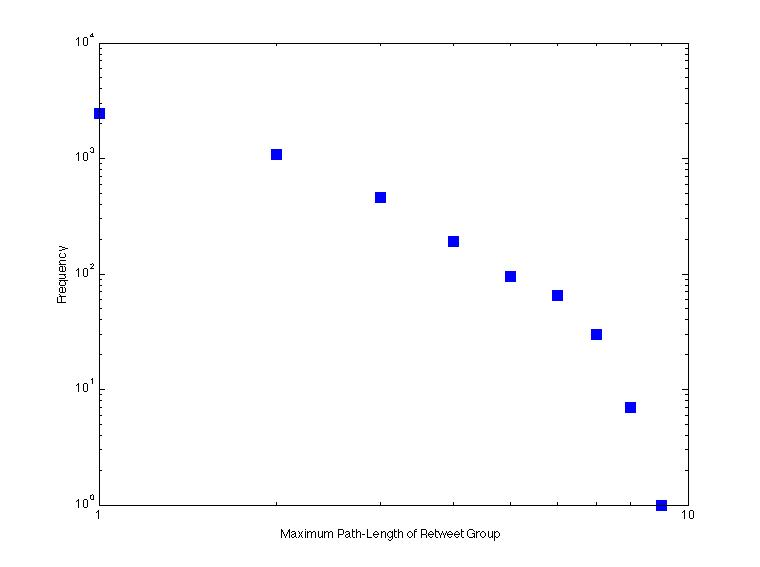
\includegraphics[scale=0.35]{4.Chapter1/Media/pathlength-distribution.jpg} 
\caption{\textit{Log/log distribution of maximum path-lengths from retweet groups.}}
\label{fig:pathlength-distribution}
\end{figure}
It should be noted that the very high proportion of single-chain path-lengths could be a result of the new method of retweeting introduced in the previous section, since, as mentioned, if all of the users in a retweet chain were to retweet in this way then Twitter would still only treat the path-length as one; between the original tweeter and each of the intermediate retweeters. Despite this, the result fits the rest of the dataset well.\\
This data can also be used to have a look at the friend-follower graph associated with retweets. In cases where the group's maximum path-length is equal to one (i.e. simply the case where a user has retweeted another user's tweet once), the retweeter follows the original tweeter about 90\% of the time. This implies that in 10\% of cases, a retweeting user has retweeted a tweet found outside of their home timeline, i.e. on the public timeline, or whilst browsing through other users. It could also be as a result of the retweeter not including the tweet citation (`@username') for reasons such as to save space, which would be particularly likely in cases of longer tweets. This implies that the more followers a user has, the greater chance that user has of having his or her tweets seen and of being retweeted. Since 90\% of retweets occur if the retweeting user follows the original tweeter, then this is directly demonstrated. However, this does not take into account whether the tweet was passed down a chain of retweets retweeted with the second (single click) method. In these cases the path-length would be represented with a length of one even if they were actually longer. The introduction of the second method of retweeting is, therefore, not helpful with the analysis of retweets.\\
In addition to this, in cases where the maximum path-length is greater than one (i.e. at least one user retweeting in a chain between original tweeter and final retweeter), the final retweeter follows the original tweeter in about 40\% of cases. From Figure \ref{fig:totalretweets-pathlength} we can see that retweet groups with a larger maximum path-length tend to be larger themselves. This means that the tweet has travelled further both around the original tweeter, but also potentially to other communities. Users from other communities will be less likely to follow this original tweeter, explaining this drop in likelihood. Results have also hinted that the probability of users citing the original tweeter decreases as the path-length of the retweet increases, which also goes some way to explain this point. 

\subsection{Size of Retweet Groups}
\label{size of retweet groups}
This section focuses on properties of retweet group size, and also how this can be related to path-length. The average retweet group size found from the data was of size 6, with the largest and smallest retweet groups being of size 284 and 2 respectively.\\

The distribution of retweet group sizes can be seen in Figure \ref{fig:retweet-distribution} and shows that this data follows a power-law distribution (with a relatively large \textit{p}-value of 0.871). The $Pr(X \geq x)$ represents the complementary cumulative distribution function, where the randomly generated \textit{X} is greater than or equal to \textit{x}. These values were calculated using the techniques and code provided by \cite{clauset07}.\\
In these retweet groups, and particularly the larger ones, retweets are likely to be down several chains. Combining this information with that of the average path-length of retweets, it becomes more clear how the retweet tree structure is created, with nodes being the retweeting users (the root node being the original tweeter), and edges between nodes being the path of retweets. Different retweet chains would be illustrated by the combinations of journeys down different branches. The longest path-length would be represented by the depth of the longest tree branch, and the total number of retweets would be represented by the number of edges. The trees can be said to represent the retweet groups, though, in practice, many members of the group will be separate from the main tree due to missing citations.\\
\cite{kwak10} discusses retweet trees in more detail, in particular, the different shapes of the trees representing retweet groups from the Air France incident. Their results, for these trees, also (see section \ref{length of retweet chains}) indicate a large number of groups with maximum path-lengths of one and two.\\
\begin{figure}[h]
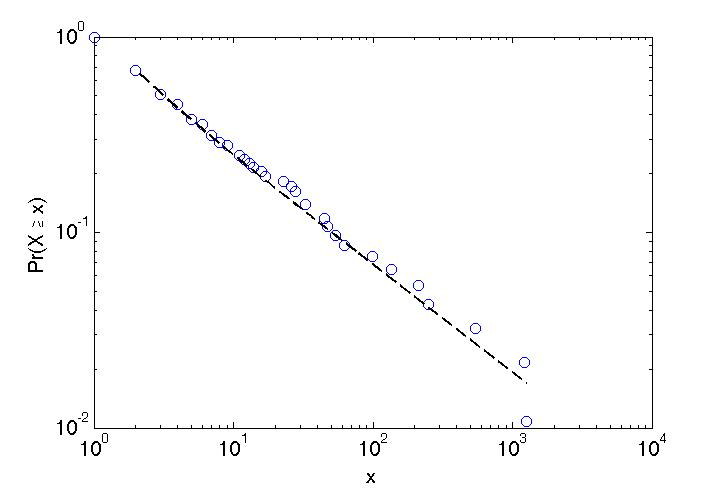
\includegraphics[scale=0.35]{4.Chapter1/Media/retweets-distribution-stats.jpg} 
\caption{\textit{Maximum likelihood power-law fit for the cumulative distribution of retweet group sizes.}}
\label{fig:retweet-distribution}
\end{figure}
\begin{figure}[h]
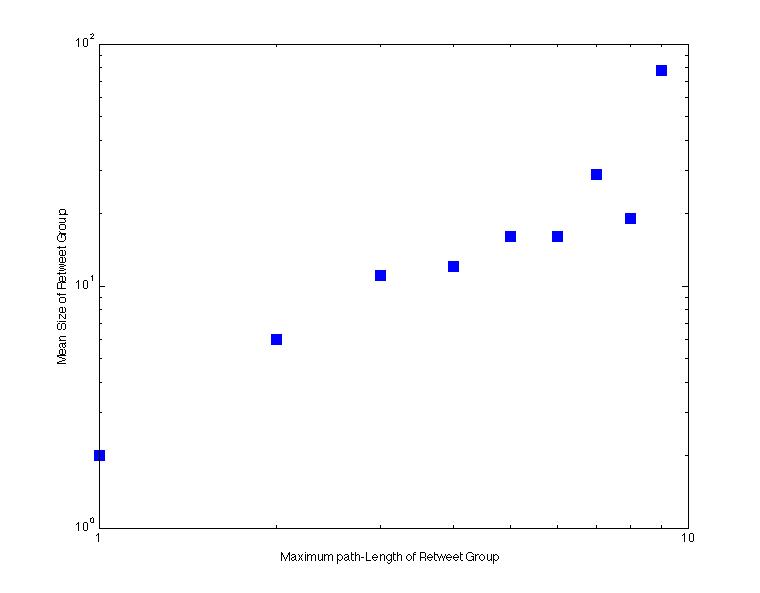
\includegraphics[scale=0.35]{4.Chapter1/Media/retweets-pathlength.jpg} 
\caption{\textit{Log/log relationship between the maximum path-length and size of a retweet group.}}
\label{fig:totalretweets-pathlength}
\end{figure}
Figure \ref{fig:totalretweets-pathlength} shows how the total number of retweets varies with the longest path-length of the retweet group. The trend mostly correlates with what might be expected; that the maximum path-length of a group increases with the overall size of the group. These illustrations do not show which users are followers of others, but do show how some tweets are retweeted significantly more than others. Users who have many more followers are said to be more \textit{influential}, say Cha M. et al. \cite{cha10}, who also discuss the idea of `indegree', and that those users who have far more followers than friends are likely to be far more influential. Their chance of having tweets retweeted is therefore increased.\\
The (immediate) audience size of a retweet group refers to the number of users the tweet has been exposed to either directly or through retweets. \textit{Immediate} was used in this sense since users who have made their profile public can have their tweets viewed by users who aren't followers of the former. This audience size can therefore be calculated simply by summing up all the followers of each of the users in the retweet group.\\
\begin{figure}[h]
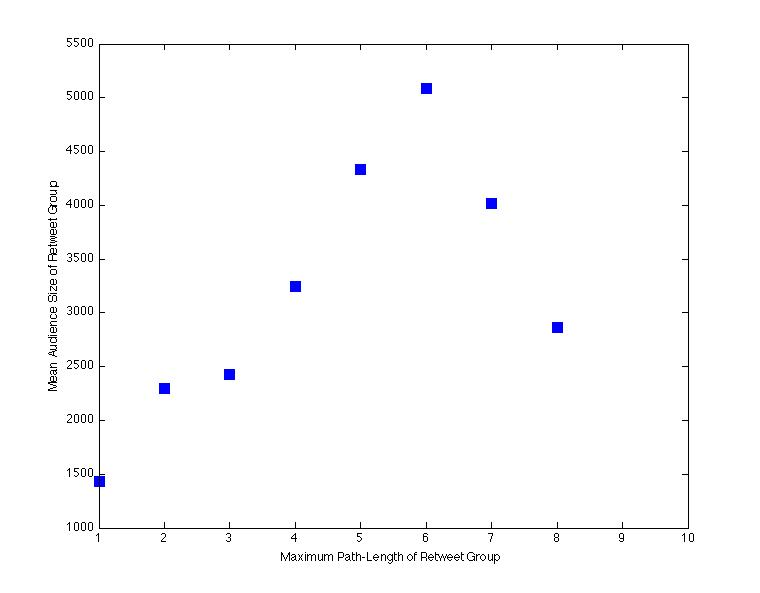
\includegraphics[scale=0.35]{4.Chapter1/Media/audience-pathlength.jpg} 
\caption{\textit{Relationship between a retweet group's audience size and its longest path-length.}}
\label{fig:pathlength-audience}
\end{figure}
These audience measures take into account that some users may be exposed to the same tweet more than once. This happens when users involved in a retweet tree have some followers in common, and so is likely to be prevalent in more closely-knit communities. As a result, the audience sizes shown only represent \textit{distinct} users exposed to the tweet.\\
Collection of the audience size from the data started slightly later than the main dataset and is only available for 2860 of the total 4400 groups. The longest maximum path-length of this subset is 8.\\
Figure \ref{fig:pathlength-audience} shows how the audience size of retweet groups varies with their maximum path-length. The peak at path-length 5 indicates that the groups with a mid-range maximum path-length tend to have a larger audience size, and we believe this is to do with the amount of audience overlap in different retweet groups.\\
\cite{kwak10} discusses how retweeting is related to the audience size of a tweet and how the power of the retweet phenomenon can greatly affect the spread of information, even if the original tweeter has only a few followers. The same paper more specifically mentions that the audience size of a retweeted tweet reaches, on average, at least 1,000 users, no matter the number of followers of the original tweeter. This can also be seen in our results; that no matter the maximum path-length of a tweet, the number of users reached is relatively high.\\
The overhead of a retweet group represents the number of users who are exposed to a tweet more than once and is present in 71\% of retweet groups. The \textit{proportionate} overhead is the ratio of overhead to audience size and the mean of this was found to increase with the group's maximum path-length. This is a possible explanation for the peak in the data: that eventually the overhead of non-distinct users has increased to the extent that it reduces the audience size more significantly. The same graph representing the effective audience size (calculated with the addition of non-distinct users) represents, mostly, a continuous positive correlation.\\
Three of the largest five overheads collected were from retweet groups with a maximum path-length of 1, the largest with an overhead of 6.5 times greater than the distinct audience itself (the overhead was larger than the actual audience size in around 3\% of retweet groups). This shows that, to an extent, there can be significantly more overlap in more closely-knit communities; those retweet trees which are wide and shallow. The chance of getting no overhead increases in smaller retweet groups.

\subsection{Retweet Follower Pattern}
\label{retweet follower pattern}
This experiment focuses on the pattern of followers in the retweeting hierarchy.\\
The first result shown from the experiment is that the final retweeter follows the previous retweeter in the chain in 67\% of cases. It initially seems strange that this should be 20\% lower than when following a user in retweet chains of length one. This suggests that users involved in shorter-chain path-length retweets are members of more tightly-knit communities. Retweets with longer path-lengths have, by nature, travelled further and so would be the type of retweet to travel between communities, reducing the chance of the involved users following each other.\\
The interesting part of this, however, is the number of followers of the previous retweeter in different cases. In the 33\% of cases where the final retweeter doesn't follow the previous retweeter, the latter has, on average, around 600 followers. When the final retweeter \textit{does} follow the previous retweeter, however, the previous retweeter's average number of followers is 940. This is quite a substantial difference and certainly highlights the fact that by having more followers you are more likely to have more influence in terms of whether you get retweeted, or not.\\
This is accentuated further when looking at the original tweeter. The likelihood of a retweeter following the original tweeter in cases in which the path-length is of more than one has already been found to be around 40\%, but the average number of followers of the original tweeter increases by a factor of around four (580 to 2000) when also followed by the final retweeter. Results showed that the original tweeter had a consistently higher number of followers when followed by the final retweeter than when not at all path-lengths. This demonstrates that having an increased number of followers is correlated with the chance of a user being retweeted. In this case, having four times the followers increases the correlation dramatically (40\% to 90\%). The number of followers of a user can therefore be directly related to the ideas of influence discussed in \cite{cha10} and also of `advertising' themselves.\\
\begin{figure}[h]
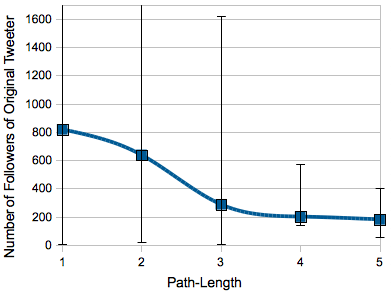
\includegraphics[scale=0.6]{4.Chapter1/Media/originalfollowers-pathlength-distribution.png} 
\caption{\textit{Relationship between number of followers (and respective distribution) of the original tweeter as the path-length increases.}}
\label{fig:originalfollowers-pathlength}
\end{figure}
It was found, however, that the number of followers of the original tweeter diminishes as the path-length of the tweet increases (Figure \ref{fig:originalfollowers-pathlength}), signifying that tweets travel further when the original tweeter has fewer followers. Because the retweet groups were collected in such a way so that groups containing longer path-length retweets also contained many shorter-chain retweets, retweet groups containing path-lengths of 5 (or more) are also likely to contain many retweets (if not more) with path-lengths of one or two (see the distribution in Figure \ref{fig:pathlength-distribution}). It can therefore be argued that there are more users involved in shorter-chain retweets than in ones with longer path-lengths. It is then more likely for these users to have more followers than others in the retweet group. Another explanation could be that users are actually aware of their local network and realise that retweeting may cause a lot of audience overlap (particularly in the case of large communities). A user may have seen a post retweeted a few times on their home timeline and thus decide not to also retweet.\\
One last interesting point to make regarding the notion of retweet chains is looking at the how the pattern of following previous retweeters develops as the path-length increases. It has already been discussed above how the chance of following the previous retweeter in the chain is about 67\%, but, in cases where the path-length of a tweet is greater than two (i.e. at least two intermediate retweeters between final retweeter and original tweeter), the chance of the final retweeter following the next retweeter along preceding the previous retweeter is around 45\%. This suggests that retweeting is more widespread and not so much just circulated around communities. These preliminary results demonstrate that the chance of the final retweeter following previous retweeters - up to and including the original tweeter - diminishes along the chain or as the tree is ascended (Figure \ref{fig:following-possibility}).\\
\begin{figure}[h]
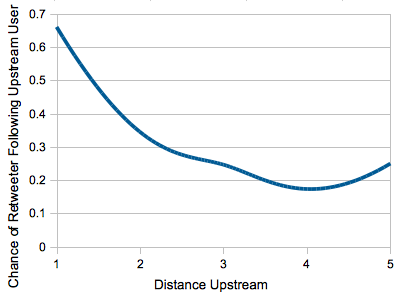
\includegraphics[scale=0.55]{4.Chapter1/Media/following-possibility.png} 
\caption{\textit{Proportion of final retweeters following upstream users at varying distances along the chain.}}
\label{fig:following-possibility}
\end{figure}
Because of this, it's sensible to assume that the tweets in the dataset are forwarded through less-connected users, and perhaps forwarded from community to community by those users belonging to several groups. Otherwise, if the retweets were circulated more around closely-knit communities, the likelihood of the final retweeter following the previous tweeters would be both greater and more evenly spread - i.e. the chance of following the previous retweeter would be roughly equal to the chance of following the other tweeters in the chain.\\
In addition, of the 67\% of final retweeters who \textit{are} following the previous retweeter, about 19\% of them also follow the next previous retweeter (i.e. the retweeter at path-length - 2). In this case, the next previous retweeter has, on average, 3000 followers. In the 81\% of these users \textit{not} following the next previous retweeter, then the latter has an average of 525 followers. This is an accentuated result of the one previously, but this time boasts an increase of a factor of 6.\\
Of the 33\% of users who \textit{don't} follow the previous retweeter, about 30\% follow the next previous retweeter. Both of these sets of statistics also go towards the idea of the diminishing chance of following the users as the tree is ascended.\\
From this dataset, it was also possible to work out how often retweeters cited the original tweeter of a post. In retweets, users are typically cited by, as we have seen, having their name along with an `RT' at the start of the post. This data was collected by seeing if the original poster's username was mentioned \textit{anywhere} in each retweet. The chance of this occurring was found to be around 68\% and did not vary with any pattern with path-length.
 
\subsection{Retweet Time Delay}
\label{retweet time delay}
The final experiments in this section focus on the time delay between the final retweeter and original tweeter. This is an interesting area since it enables researchers to see how fast messages propagate through the Twittersphere. From this information, and by using the retweeter patterns demonstrated above, it would be possible to work out how far and how quickly information can be passed around.\\
Figure \ref{fig:timedelay-pathlength} shows the average time delay between the first and final retweet with increasing maximum path-length of the retweet group.\\
\begin{figure}[h]
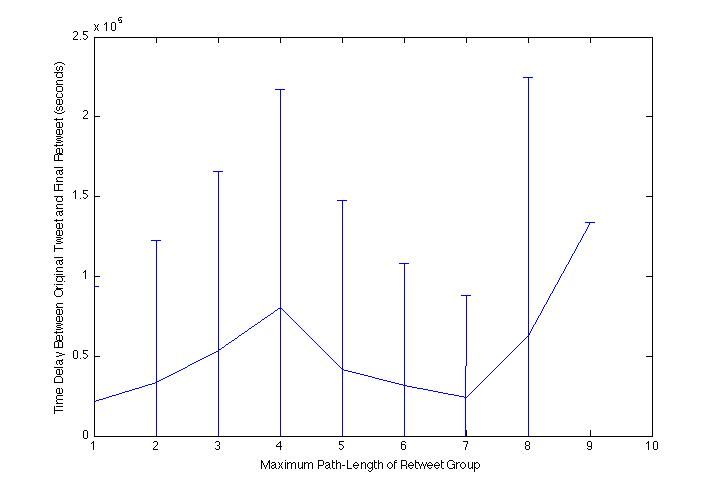
\includegraphics[scale=0.35]{4.Chapter1/Media/pathlength-timedelay.jpg} 
\caption{\textit{Average time (in seconds) between first post and final retweet of a retweet group varying with the group's maximum path-length.}}
\label{fig:timedelay-pathlength}
\end{figure}
The results indicate that, mostly, as the group's maximum path-length increases, then so does the elapsed time between the original post and the final retweet. This is probably as was expected, since this shows that it takes longer for a retweet to travel further. The data is not consistent, however, especially results for a path-length of five and above. The first four results suggest a uniform incline roughly proportional to $ v=\frac{s}{t} $, where the distance, \textit{s}, is the hypothetical distance given by the path-lengths, showing that the \textit{speed} of propagation remains mostly constant.\\
There is not enough of a trend in the data to make any deductions regarding propagation speed, however. There are two main conflicting arguments regarding this result: the first is, as mentioned, that the further a tweet travels the longer time it travels for. The second is to do with tweet popularity: the more popular a tweet is, the more quickly it will be retweeted. In the latter case, it is possible that longer trees grow fully before shorter ones, implying exponential growth. Generally, though, it seems that the maximum path-length of a retweet group does not massively affect the tweet's propagation speed.

\section{Summary}
\label{analysis}
The experimental results have certainly highlighted the ideas of communities and that of message cascading similar to that demonstrated in \cite{java07} and \cite{galuba10} respectively.\\
As has been seen, in section \ref{retweet time delay}, the retweet tree seems to grow in a variety of ways. One argument is mostly expected; that as the `distance' the tweet travels increases, then so does the time taken for it to reach its end. The other argument is linked to the idea of tweet advertising, discussed in previous sections, and namely the notion of tweet popularity.\\
The previous experiments showed how the number of followers of a user directly influences their chance of being retweeted. It can therefore be seen that advertising can also be linked to the level of influence a user has. The results help illustrate the multi-dimensional properties of the retweet tree, and how these factors relate to its growth and its associated friend-follower graph.

%\section{Conclusions}
This paper has demonstrated relatively simple results in an attempt to realise some of the behavioural patterns of retweets, both linking to the psychologically in terms of the users, but also the physical properties of retweets. The results are able to represent a basis for potential further work and research into the various aspects of Twitter, moreover, perhaps, topical categorisation and the dynamicity of the friend-follower graphs.

\chapter{Analysis of Twitter's Social Structure}
\chapter{Analysis of Twitter's Social Structure}


Stuff to add to this section:
\begin{itemize}
\item Change tweet features for each simulation and make comparison on these differences
\item Observe differences in patterns when network generation parameters are altered
\item Link up section to previous section (i.e. how did the previous research help and how does this build on that work?)
\item Explain how this section becomes the basis for work in 'main chapter 3'.
\item (e.g. Issues with current method (too long, requires network, inaccurate due to having to choose users with fewer followers), so need a quicker, more accessible and online approach).
\item Explain the Mechanical Turk questions in more detail, with examples.
\item Discuss about the machine learning approach used (logistic regression and how it works)
\item Link 'retweet volume' to 'retweet group size'
\end{itemize}

Twitter is often seen as one of the biggest sources of new and live information on the Internet, with millions of people producing and absorbing information daily. Users receive tweets onto their timelines from the users that they follow. Thus, a user has some control over the \textit{type} of information they receive by choosing which other users to follow. A particular user, therefore, may not be aware of information that exists outside of their local network, since he or she is not directly exposed to the information produced by non-followees.
\\
Retweeting allows users to forward information they receive onto their own followers. As a result, followers of these users, who might not normally be exposed to this information, now have a chance to access it. A user who decides to retweet a tweet can be said to consider that tweet to be \textit{interesting} (at least, to their followers), since that user has taken the time to read the tweet, decided whether or not to share it, and then to actually retweet it \cite{uysal11}.
\\
Several factors can affect a user's decision to retweet, such as whether the tweet contains an (interesting) URL, whether the tweet mentions another user, whether a user even has a chance to see the tweet, the influence of the author, and so on. These factors account for a user's individual retweet \textit{decision} on a particular tweet, and the combination of several users' retweet decisions dictate how far the tweet will propagate. However, it is our belief that the social network structure also has an affect on how far tweets can travel.
\\
The social structure of Twitter is built up by users electing to follow other users. When a user follows a user, a directional link is forged between them, and any tweets generated, or forwarded, by the followed user are passed down the link. It's clear to see that, as more links are made between users, many more avenues are generated for message propagation throughout the social structure. Users with a high in- and out-degree can become an information highway, but users with a low out-degree are a bottleneck of information. 
\\
In this chapter, we demonstrate how different network types support different propagation characteristics through the use of a model simulating each network type. Using the model, we make predictions on the retweet outcomes on several network types, and compare these to the characteristics of the propagation in real Twitter networks. We finish by discussing how the \textit{interestingness} of a tweet may be inferred from simulating the network in this way.

\section{Background to This Area}
\cite{uysal11} discusses an idea similar to that of predicting the interestingness of a tweet, but focuses mainly on predicting the users most likely to find the tweet interesting enough to retweet. Similarly, \cite{hong11} looks at the same issue, but at the other way around by predicting the \textit{type} of tweets that are likely to be retweeted many times. Discussions on the retweet decision in relation to a user's recognition of its features take place in \cite{chorley12} as well as conclusions about the effect of features such as the number of followers of a user or any pre-existing metadata on the interestingness of the tweet.
\\
The notion of time decay and how this is associated with a user's retweet decision is discussed in addition to a retweet probability prediction in \cite{zhu11} (and \cite{peng11}), which is the basis of the model we use in this paper.

\section{Overview}
In the next sections, we introduce and briefly explain the regression model we use for simulations and predictions. We then go on to analyse the differences in the propagation characteristics between three different network types before comparing the results of simulations on these networks with data collected from the Twitter social graph. We finish by introducing a methodology for predicting the interestingness of a particular tweet to a particular user and how this might be improved.
\\
Ideally, there are two things we'd like to see from the first set of experiments; firstly, that changing the network type and properties does, indeed, affect the propagation behaviour, and, secondly, that at least some of the results from the experimentation correspond to Twitter's own retweet behaviour so that a fair comparison and justifications of our results can be made.
\\
With regard to our prediction work, we'd like to be able to make relatively decent predictions on which tweets are of interest, and which are not, based on the simulation research in the next section.

\section{Model} 
As mentioned above, \cite{zhu11} introduced and discussed their prediction model, which was shown to perform well when predicting the retweet decision of a user. Their model trains a logistic regression using a set of user-, tweet- and context- features in order to classify an experimental tweet and output a retweet probability based on a set of features.

\subsection{Machine Learning}
Machine learning techniques are useful for making predictions based on certain input criteria based on the perceived history of previous outputs from the same inputs. 

\subsubsection{General Overview}
For example, consider the three attributes, A, B and C, each of which is of a boolean data type. A machine learning technique is `shown' that in every case where A is True and B is False, then C is true; and that in each case where A is False and B is True, then C becomes False. The history of these inputs suggests that A is strongly associated with C (the strength of this relationship will increase if the input/output history is larger), such that if the technique now tries to predict C based on the fact that A = True, then it will likely suggest that C is also True with high confidence.
\\ \\
A technique that has been shown many of these input/output combinations (known as `instances') is said to be a trained model, where the model type is that of the learning technique used. This model can then make predictions based on the same inputs it has been trained on, and will therefore not work for attribute inputs that it hasn't been trained with.
\\
Generally, in large enough datasets, the training data will not exclusively contain instances where A is the inverse of B, and so the model will be able to make predictions in cases where A = B (though if these cases are less prevalent then the confidence of these prediction outputs will be weaker). When training the model, instances must contain the input attributes as well as the value of the output attribute. When testing against the model after training, the model is supplied the input attributes and predicts the value of the output attribute. Generally, the model will also indicate how confident it feels that the prediction is correct, and thus an idea can be obtained of the value of each of the input attributes. Some model types (particularly regressions) output instead the \emph{probability} with which the attributes align to the trained regression.
\\ \\
In this example the focus has been on boolean data types, but most machine learning techniques are not limited to these. Indeed, most applications require the learning of real numbers (integers, floats, etc.) and more highly-dimensioned nominal attributes, where there are several categories that the value of one of the input attributes can lie in. Many machine learning techniques exist and some are more accurate than others when it comes to different data types and several support the notion of `weighting' attributes, in which a strength weight is assigned to each attribute to signify the confidence with which the model should rely on that attribute for producing the prediction.
\\
For example, for purely nominal values, then logistic regressions can be accurate in predicting outcomes, whereas for a mixture of real and nominal attributes a Bayesian attempt might be more suitable. 

\subsubsection{Logistic Regression} 
The work in this chapter utilises a logistic regression for outputting retweet predictions based on the feature input criteria discussed later.
\\
As mentioned, the logistic regression predicts the statistical likelihood that the input features align with what the model has been trained with. The work in this chapter relies on the use of a retweet probability of a given user acting on a given Tweet at a certain time. Thus, it is trained in such a way so that the binary input attributes produce a binary output retweet outcome attribute: 1 for retweet, 0 for no retweet.
\\
When testing, the binary features of the test set are used to output the probability that these features will result in a retweet.

\subsection{Algorithm}
Include image indicating the flow of events that take place for the model
\\
Pseudocode for the algorithm
\\
In essence, the model requires a network of users and one tweet to start the simulation. It starts by initialising a user set, \textit{U}, to contain one source user from the network, $U_s$. This source user then transmits a tweet which is then received by its followers. $U_s$ is then removed from $U$. For each follower, its tweet and user features are classified to produce a retweet probability. If this is greater than a random number, $R$, then the user retweets the tweet to its followers and the process repeats. Any user that retweets the tweet is removed from $U$ and added to the retweet decision set $RT$. The followers of the retweeter are added to $U$ for the next iteration, in which each user in $U$ has received the tweet onto their timeline. The retweet volume of this tweet in this network is then the cardinality of the set $RT$.

\subsubsection{Twitter Timelines}
A tweet in a user's timeline will slip further down in the timeline as time goes by. This happens whether the tweet is interesting or not and whether or not the user has even seen the tweet.  Users having a quick browse through Twitter may not have time to scroll down to find these interesting tweets (and will not know they exist) and thus tweets left in the timeline have their retweet chance decay over time.
\\
We emulate this phenomenon in our simulations by removing the tweet from a user's timeline (by removing the user from the set $U$) if the user has not retweeted the tweet within a timestep threshold, which can be varied to alter the volatility of the retweet.

\subsection{Features}
We use this model as part of a simulator in order to obtain an approximate retweet volume of each tweet when the retweet probabilities of each user receiving the tweet are combined. \cite{zhu11} used a set of around 50 features, though they mention how some features have more weight than others. In order to simplify the simulation significantly and to make data collection more tractable, we decided to use only the following four major features;
\begin{itemize}
\item \emph{follows} - Whether or not the user exposed to the tweet is a follower of the author;
\item \emph{followed} - Whether or not the user exposed to the tweet is followed by the author;
\item \emph{mentioned} - Whether or not the user exposed to the tweet is mentioned in the tweet;
\item \emph{URL} - Whether or not the tweet contains a URL;
\end{itemize}
Where \emph{author} is defined as the user who originally tweeted the tweet.
\\ \\ 


\section{Training the Model}
\subsection{Data Collection}
To collect the training data, we crawled Twitter, using the REST API, from March-June 2012 to collect a set of around 12,000 tweets and retweets from the Twitter public timeline. In addition, we made further calls to collect the information required for the features (namely the \textit{following} and \textit{followed} features). 

\subsection{Feature Extraction and Regression Training}
FILL THIS IN
\\
The above features were extracted in each case and the regression was trained.


\section{Network Analyses}
In this section, we look at three different network structures and discuss the differences in the propagation patterns produced by each. Note that each graph we assess is \textit{directed}. The same set of tweets are used for each simulation on each of the networks.

\subsection{Path Network}
A path network is the most simple of the three, and is also the least life-like when compared to Twitter's own social graph. In this network, the output retweet volume is, by definition, equal to the penetration (i.e. \emph{depth} of propagation) of each tweet.
\\
In this case, a directional path network consists of a network of users, $ N $, of size $ n $, in which each user $ N_i $ is followed by user $ N_{i+1} $ for $ 1 \le i < n-1 $. As a result, all users in the network, except the user $ N_n $, have precisely one follower.
\\
Since each internal user only has one follower, the likelihood of a retweet occurring at each timestep is somewhat reduced, it is expected that the retweet volume will tail off more soon than in other network types. Propagation is also hindered by the fact that each retweet can reach an audience with a maximum size of 1 at each stage, thus relying on that single user making the retweet.
\begin{figure}[h]
\centering{
\begin{tikzpicture}
 \begin{semilogyaxis}[
        xlabel=Retweet Volume,
        ylabel=Frequency,
        grid = major]
    \addplot[only marks,mark=*,blue] plot coordinates {
        (1,540)  (2,118)  (3,53) (4,27) (5,13) (6,5) (7,4) (8,2) (9,1) (10,0)
    };
\end{semilogyaxis}
\end{tikzpicture}
\caption{Retweet volume frequency distribution from path network simulation}
\label{fig:linear}
}
\end{figure}
Figure \ref{fig:linear} shows the frequency distribution for a path network when simulated with the logistic regression over a series of tweets. The graph shows a very large proportion of single retweets, which reduces logarithmically with larger volumes.
\\
The likelihood of a user getting the chance to retweet, and also deciding to retweet, becomes the product of a probability function the further the tweet travels, where user $ N_i $ requires all users $ N_0 $ to $ N_{i-1} $ to pass on the message before it even gets a chance to make the retweet decision.
\\
As a result, if the retweet decision chance of each user is more or less equal, the chance of user $ N_2  $ retweeting the tweet is of an order of magnitude less than that of user $ N_1 $ deciding to retweet. The graph shows half life-style behaviour; owing to the fact that each retweet is exponentially less likely to occur than the previous retweet. Note that the graph is plotted on a log-linear scale.

\subsection{Random Network}
Random networks are more similar to Twitter's own social structure than path networks, but are a much more basic and uniform version and do not consider more influential users or the development of Twitter communities.
\\
A random network is defined as a network of users, $ N $, of size $ n $ in which a user $ N_x $ has probability $ p $ of following user $ N_y $. Thus; as the probability $ p $ is increased, the likelihood of a user following other users in $ N $ increases, causing the overall network edge density to increase. Generally, the average number of followers and followees of a user is proportional to $ p\times n $. Thus the parameters for constructing such a graph are the network size, $n$, and the attachment probability, $p$. The simulation results for the random network indicates a higher distribution of mid-range retweet volumes.
\begin{figure}[h]
\centering{
\begin{tikzpicture}
 \begin{semilogyaxis}[
        xlabel=Retweet Volume,
        ylabel=Frequency,
        grid = major]
    \addplot[only marks,mark=*,blue]
       file {5.Chapter2/data/random.dat};    
\end{semilogyaxis}
\end{tikzpicture}
\caption{Retweet volume frequency distribution from random network simulation}
\label{fig:random}
}
\end{figure}
\subsection{Scale-Free Network}
Include more mathematical analysis of scale-free networks (in general) - i.e., in what way are they logarithmic?
\\
A scale-free network is a network of users, $ N $, of size $ n $ and is generated in such a way so that the resultant distribution of degree follows a power-law. \emph{In}-degree signifies the number of inward edges to a node (i.e. the number of followers of a user), whereas \emph{out}-degree is the number of outward edges (i.e. the number of users that user follows).
\\
Scale-free networks have been the subject of a fair amount of research, and are explained more thoroughly in \cite{hein06}. In our implementation we use NetworkX\footnote{http://networkx.lanl.gov}, a Python networking package, to generate directed scale-free networks through a preferential-attachment algorithm based on the network size and edge density as parameters.
\\
Figure \ref{fig:real-scalefree} shows the frequency distribution of retweet volumes. Since the data is plotted on logarithmic scales, we see a logarithmic trend very similar to our results in \cite{webberley11}.
%\begin{figure}[h]
%\centering{
%\begin{tikzpicture}
% \begin{loglogaxis}[
%        xlabel=Retweet Volume,
%        ylabel=Frequency,
%        grid = major]
%    \addplot[only marks,mark=*,blue]
%       file {data/scale-free.dat};
%    
%\end{loglogaxis}
%\end{tikzpicture}
%\caption{Retweet volume frequency distribution generated in scale-free networks}
%\label{fig:scale-free}
%}
%\end{figure}
\subsection{Comparison to Real Twitter Data}
In our previous work, \cite{webberley11}, we captured and analysed data which contained results on the distribution of retweet group sizes. In that paper, a retweet group was defined to be a set of tweets containing one tweet and then all the retweets of that tweet. Thus the retweet volume looked at in this section is effectively the cardinality of the retweet group (minus one). Since the results in the above experiments also look at the frequency distribution of retweet volumes, then we should be able to draw some comparisons.
\\
We compared the data produced by the different types of network to this previous data, and found that the scale-free network produced a distribution similar to that from the real Twitter data.
\begin{figure}[h]
\centering{
\begin{tikzpicture}
 \begin{loglogaxis}[
        xlabel=Retweet Volume,
        ylabel=Frequency,
        grid = major,
        legend entries={Real data,Scale-free}]
    \addplot[only marks,mark=*,red]
       file {5.Chapter2/data/comparison-real.dat};
    \addplot[only marks,mark=*,blue]
       file {5.Chapter2/data/comparison-scale-free.dat};
\end{loglogaxis}
\end{tikzpicture}
\caption{Comparing the retweet volumes distribution from scale-free graph simulation to data from Twitter's graph}
\label{fig:real-scalefree}
}
\end{figure}

\subsection{Structure Comparison}
Each network structure has been demonstrated to show different propagation characteristics. This has shown that, in addition to a user's own retweet decision, the actual spread of a tweet depends somewhat on how the author's local network is constructed. With lots of edges in the graph, there are many more paths down which propagation can occur, increasing the number of times a retweet decision is made, and therefore an increase in the overall number of retweets occurring. The retweet decision facilitated by the model, therefore, combined with a user network give an overall \textit{retweetability} of a tweet that will vary depending on the network it's being propagated in, the source user, and the intermediary retweeters.
\\
The path network, as designed to be the extreme case, has shown to allow poor propagation. Importantly, whilst the network parameters and retweet decision had to be globally increased to obtain any sensible data from this simulation, the trend still shows how propagation down a single chain isn't hugely effective.
\\
The random network facilitated many more retweets due to the fact that users had a very similar in- and out-degree in all cases across the network. This means that each user is able to receive a lot of information, and is also able to pass on (whether an author or a retweeter) information to lots of users simultaneously in the graph. 
\\ 
Despite random networks supporting large retweet throughput (i.e. high \emph{recall} of information), the disadvantage is that the interest \emph{precision}  is much lower. This is because this type of network relies on users following a large number of other users, thus meaning that they would receive more `noise' (i.e. uninteresting tweets) than if they were more limited and selective. Although tweets that are retweeted are usually of a higher \emph{quality}, not all retweeted tweets will be interesting to all users.
\\
Finally, the scale-free network, whilst not having the highest throughput of information, does have trends most similar to the data on retweet distributions collected from Twitter's social graph. This is due to its ability to emulate more influential users and areas of dense communities (as discussed in \cite{java07}). These networks have the potential to allow for large numbers of retweets, especially if they are sourced from one of these more dense areas, but typically die off more quickly as the tweets are retweeted through less influential users.

\section{Interesting Additional Findings}

\subsection{Graph Density}
Define edge density (with equation

\subsection{Results}
Show links between follower audience -> local network -> density.

\subsection{Uses}
From this data, it is demonstrable that various parameters can be generally successfully inferred from very basic user information.

\section{Predictions From the User Graph}
The final part of this paper focuses on the ongoing development of a method to predict the interestingness of a tweet based on the work in the previous sections. The prediction method, at a high level, compares the predicted retweet outcome of a given tweet to the number of times that tweet has actually been retweeted. If, for example, a tweet is simulated with the help of the model and produces a prediction of two retweets, but the tweet has actually been etweeted four times, then we can infer that this tweet is more interesting (at least, to a subset of users). 
\\
The tweet and user features we looked at earlier in this paper are very static, binary features, which do not take into account the actual content of the text of the tweet. Therefore, if a tweet is retweeted more than was predicted, then there is something in the tweet, such as a link to a particularly interesting article or a breaking news story, that makes it more interesting than the average tweet, with the same binary features, that was used to train the model.
\\
In order to improve the fairness of the experiment, we wanted to ensure that the environment of the tweets (i.e. the user network they are propagated through) is the same as its real-life Twitter counterpart. We could then choose a user, which would become the source user, $U_s$, in the set $U$, and simulate that user's own tweets within their particular local network as described by the model above. This would then produce a retweet volume for this user's tweets, to which we could compare the number of times that tweet has \emph{really} been retweeted.


\subsection{Data Collection}
Due to the exponential scaling properties of Twitter's social graph, it was infeasible to collect any more than two hops away from each user as a representation of that user's local network under the rate limitations of Twitter's REST API. 
\\
In particular, a single Twitter account running an instance of an application was allowed, at the time of these experiments, a maximum of 350 REST API calls per hour. One call would be required, for example, to obtain up to 5000 of the followers of a particular user (i.e. one follower hop from the user). An additional call would then be required to collect each of that user's follower's followers (in order to obtain the \emph{second} hop from the source user). \\
Thus, a user who has 700 followers would require 700 API calls to collect that follower network, in addition to the one required to collect that source user in the first place, and would therefore take over two hours of collection. To collect the \emph{third} hop from the source user would drastically multiply the number of required requests (even if there is significant overlap between the followers) and the time needed. 
\\
If each of the 700 followers of the source user had, on average, 200 followers, then this would require the gathering of $ 700 $ x $200 = 140,000 $ users, equating to more than 402 hours of data collection. Bearing in mind that this would only collect the network features for \emph{one} user, it is clear to see how this is an impractical approach.
\\ \\
Luckily, in \cite{webberley11}, we found that the vast majority of retweets occur \textit{within} two hops of the source user (i.e. a path length of less than three), so we considered that the distance from the source user in each case would be sufficient.
\\
In June 2012, the Twitter REST API was used to conduct a random walk through the social graph. For each user, we collected the most recent 300 tweets (including each tweet's metadata - particularly their retweet count) and their local follower network within two hops. We didn't collect the friend network, as we were only interested in tweets propagating outwards from the source user.
\\
After processing that user, the walker chose a user at random from the present user's set of followers and made this the new current user from which to collect data for. If the present user, at any stage, does not have any followers, a list of previously accepted users is maintained and a follower is chosen from one of those instead.
\\
The walker continued until the rate limit was met, at which time the current state was written to disk, and the walker waited until the rate limit was reset before continuing.
\\
Generally, this resulted in, for each user, a set of up to 300 tweets (totalling to around 10,000 tweets in total) and the network in which these tweets were propagated within. There was no need to collect any further data to train the regression, since we were able to re-use the trained model we used earlier.



\subsection{Validating Results}
Needed to validate results using human input. Machines themselves are generally unable to express human interests, so results need to be properly evaluated.

\subsubsection{Crowdsourcing}
Discuss crowdsourcing, its uses, how it is useful in this area. Talk about its history (with any references), and then about mechanical turk.
\\
Mention mechanics of mechanical turk, how it is US only (but we used crowdflower - which autmatically handles submission to MT and several other crowd-sourcing services.

\subsubsection{What We Wanted to Assess}
Used MK, etc.

\subsubsection{Constructing the Questions}
Set up questions (i.e. 5 tweets - choose most interesting and least interesting), give example of this.


In order to validate our prediction results, we ran a pilot user study in order to obtain some human input on the interestingness of each tweet. We compiled the tweet data into a set of questions which were submitted to Amazon's Mechanical Turk. Each question consisted of five tweets from our dataset and each Mechanical Turk Worker (MTW) undertook five questions. Each question asked the MTWs to select which tweet was the most interesting of the five, and which was the least interesting.
\\
For consistency we ensured that at least three MTWs had answered each question. When selecting tweets to include in the Mechanical Turk questions, we excluded those which are `@-replies' - i.e. tweets which begin with another user's screen-name and typically form part of a conversation between two or more users. This meant that there were around 4,500 tweets in total in the questions.

Through using the model and simulating each user's tweets through their individual local networks we achieved around 86\% accuracy in correctly predicting the number of times each tweet was retweeted. 
\\
The precision in predicting the \textit{interestingness} of each tweet was around 30\%. While this value is low, it does mean that in 30\% of cases, a tweet that we predicted to be interesting was verified to be interesting by at least three MTWs all selecting one tweet from a set of five. In addition, when simulating the questions by randomly choosing the most `interesting' tweet of the five in each case, the performance was unable to near our precision even after several thousand iterations.

\subsection{Improving This}
Need offline methodology.
\\
One route for this would be to try and infer a user's local network from a set of their immediate parameters, drawing on our earlier work suggesting that the Twitter network has the properties of a scale-free small-world graph. Through studying graph patterns, it is possible to make sensible inferences on the edges and nodes of a user's local network based on their follower count. From this, a graph edge density can be calculated, $ d = \frac{|E|}{|N|(|N|-1)} $, for use in generating a scale-free network.
\\
Since, for these preliminary experiments, we were only able to collect data from users with a more modest local network, the real and predicted retweet values were both relatively low, allowing more room for error. When simulating much larger local networks involving many more real retweets for each tweet, predicting interestingness, with some threshold value, may become more accurate and thus help improve the precision. The reason for this is that the retweet count of tweets that naturally get retweeted many tens, hundreds, or more times is likely to vary more with interestingness than those that are naturally only retweeted very few times.

\section{Future Work}
There is much further research that could be carried out based on the results in this chapter. Now that the foundation has been laid for simple retweet prediction based on network analysis, research could begin to look at ways in which, as mentioned, networks could be generated based on a few environmental features surrounding users.
\\
This would allow for quick generation of user networks (bypassing the need for data collection) and would also support the same calculations for more highly influential users (users with more followers and more retweets per Tweet).
\\ \\
For this research, the notion of the network will continue and form the basis of the environmental features in the next chapter. Since we now know that the network plays an important role in dictating the way in which information can propagate

\section{Summary}
In this chapter we aimed to carry out a study on the behaviour of propagation through different types of social graph structures and to introduce our ongoing work into predicting the interestingness of tweets from their retweet patterns.
\\
Using a set of tweet and user features, we trained a regression model which we used to simulate a number of tweets through different network types. We produced a distribution of retweet volumes for each network type and confirmed that, with the same tweet features, different network configurations do indeed facilitate different retweet behaviours in terms of propagation spread. We were also able to compare our results to data from Twitter to verify that Twitter's own social graph most closely resembles a scale-free small world graph.
\\
We then finished by discussing how we used the trained model to simulate real networks from Twitter, along with the tweets that were passed through these networks, in order to try to predict how interesting a tweet is based on its retweet patterns. While we were able to often correctly predict the retweet outcome of a tweet, we found that more work would be required to improve the performance of predicting whether or not these tweets are truly interesting to users.

\chapter{Inferring Interestingness of Tweets based on Information Flow Through the Network}
Introduction to online interestness inference.
\\ \\

Mention:
\begin{itemize}
\item How this chapter builds upon network stuff in previous chapter
\item We hope to compare and contrast two better ways of predicting retweet volume \emph{and} interestness
\item What needs to be improved (speed, usability - more users with more followers etc.)
\item Why do improvements need to be made?
\item How is this useful, and how does first chapter relate to work done here?
\end{itemize}

%\section{Inference Generation Using Pseudo-Networks}
%Discuss:
%\begin{itemize}
%\item Estimation of local network size from number of followers
%\item Model trained on existing dataset with features and an outcome of type boolean (true/false)
%\item Further estimation of local network \emph{density} from network size and number of followers (and shared followers, if any)
%\item Generation of estimated local network
%\item Use this network as a testbed for retweet predictions similar to previous chapter
%\item This approach uses the regression to model a particular user's retweet decision on a tweet at any one time.
%\end{itemize}

Discuss:
\begin{itemize}
\item Does not use network to simulate tweets - instead uses a set of user features
\item Previous chapter shown how basic features can be used to generate a scale-free network, which is what twitter is
\item Use these features as input attributes of a new machine learning technique model.
\item This method does not use a network or model individual user decisions
\item Trained on a set of that particular user's tweets with the retweet outcome of integer type
\item A new tweet modelled with the regression outputs a retweet volume prediction without having to simulate the Tweet's travels through the network. 
\item Discuss about the machine learning approach used (logistic regression and how it works)
\item Talk about the 'binning' of retweet outcome volumes and its approaches (distribution dependent / independent, tables of precisions, etc.)
\item Link 'retweet volume' to 'retweet group size'
\end{itemize}

\section{Background}
Stuff introducing this section and its differences to the things in the previous chapter.
Whilst machine learning was used in the previous chapter... more in depth in this area.

\section{Machine Learning}
Explain about Machine Learning, its uses, techniques and how this is useful.
\\
Talk about how it was used in previous chapter, but that more in depth here.
Bayesian Network



\section{Features}
To train the Bayesian Network model, a series of new features were harvested. Generally, each of these features fell into one of two categories; user features and tweet features.
\\
The Tweet features follow the same ideas as the features used in the previous chapter: static, generally binary features that describe the structure of the Tweet. The user (or `network')  features are related more to the \emph{network} to which the Tweet belongs.

\subsection{Data Collection}
Twitter walk, total tweets, splitting dataset, etc.

\subsection{`Twitter is a Memepool'}
Introduction to memetics (Richard Dawkins intro maybe):
\\
\begin{itemize}
\item Gene is a physical entity containing information and instructions. It is a unit of genetic inheritance (i.e. offspring typically have a mashup of the genes of the parens)
\item The result of the data held by a gene (the genome) means that organisms with certain genes are able to reproduce and survive more than other organisms containing different genes.
\item Thus the gene is able to replicate under certain gene- and environmental-centric conditions.
\item A meme is similar to  gene but is non-physical. They are a unit of cultural inheritance (an idea, phrase, behaviour, etc.).
\item Like genes, memes are able to survive better when their features (\textit{menome}) are suited to the meme's environment. In such environments, the meme is able to be shared and replicated more efficiently and frequently.
\item A Tweet, again, is similar to both. A Tweet itself has many features (the text of the Tweet, the time of its origin, its length, etc.) and their environment, the Twitter social structure, has features (namely the users that belong to it and the way they are connected) which may facilitate the replication (i.e. Retweet) of the Tweet.
\item A Tweet existing in different social structures will have different Retweet patterns, which is what we want to show in this chapter.
\item Thus tweetfeatures = genome, userfeatures=environment
\end{itemize}

\subsection{Tweet Features}
table of tweet features

\subsection{User Features}
table of user features

\section{Retweet Volumes as Nominal Attributes}
In order to try and improve the accuracy of the model at predicting retweet volume outputs, a nominal output attribute would be better than a real one. Predicting a continuous numeric value could render inaccurate results and calculating the cut-off points at which to mark as the upper- and lower-bounds for the output based on the inputs would raise difficulties.
\\
Instead, the retweet outcomes were to be `binned' into several categories which would be determined on the fly based on the outcomes present in the training data.

\subsection{Binning the Retweet Outcomes}
Describe the different methods (linear, distributed 1, distributed 2), and their advantages/disadvantages, with examples showing the graph of 
what the bins look like.
\\
Focus on the distributed 2 example, and why this is better.
`Requested' bin number not usually the same number as what is actually returned (due to large numbers of smaller retweet groups).
\\
Pseudocode

\subsection{Varying Bin Sizes}
Number of bins: explain how accuracy worsens as bin number increases.
\\

\section{Classification}
Compared several types of classifiers (show table comparing accuracy, etc. of different types)
\\
Explain that Bayesian Network is best (quick, accurate)

\subsection{Training Results}
Playing with Weka to improve the prediction performance (i.e. different number of bins, different features)


\subsection{Obtaining the Prediction Outcomes}

\section{Validating the Predictions}
\subsection{Procedure}
MK stuff
\subsubsection{Questions asked}
What did we ask
\subsubsection{Acceptance Confidence Criteria}
How many did we ask, how many classifications for each tweet, how did we split up the tweets into questions
\subsubsection{Randomised Controlled Trials}

\subsection{Results}
What were the results?

\section{Analysis}

\section{Comparisons}
\begin{itemize}
\item Comparison of two approaches
\item Which is more accurate?
\item Which is quicker?
\item Which is easier?
\item etc.
\end{itemize}

\section{Summary}
\begin{itemize}
\item Summarise comparisons - which method is overall better?
\item How does it compare to offline method from previous chapter?
\item Generally explain how the `winning' method is good and accurate.
\end{itemize}

\chapter{Critical Assessment and Conclusions}
\chapter{Critical Assessment and Conclusions}


\section{Critical Analysis of Results}
\subsection{Analysis of Initial Research}
\begin{itemize}
\item What was the use of initial research?
\item Are the results sensible?
\item How have the results shaped the further research?
\end{itemize}

\subsection{Analysis of Final Results}
\begin{itemize}
\item Have methods been able to sensibly predict retweet volumes?
\item Have methods sensibly inferred Tweet interestingness?
\item What might have worked better?
\item Which parts were useless?
\item Which parts helped develop other areas of research which may have provided further avenues of research ideas?
\end{itemize}


\section{Further and Future Work}
How can this research be taken further in the future?

\begin{itemize}
\item Use previous results to predict how far a tweet is likely to be retweeted (for advertising purposes)
\item Useful for detecting the kind of messages that are likely to travel further
\item As well as providing an interest level, the systems also predict sensible estimations on retweet volumes.
\item Perhaps useful for measuring the spread of rumours.
\end{itemize}


\section{Conclusions}
\subsection{Summary}
Summarise events and processes covered, reiterate what the point of the work was and how each part of the work covered relates to that.

\subsection{Contributions}
Restate the original contributions (from Introduction section). Explain the ways in which the work done relates to the projected contributions, that it is novel and useful.

%\chapter{Future Work}
%\input{8.Future/future-work}
%
%\chapter{Conclusions}
%\chapter{Assessment and Conclusions}
Here is provided an overview and assessment of the work conducted in this thesis, bringing together the ideas from the initial research and how these have helped in developing the methodologies introduced in later chapters. The validations from the methods are further assessed, followed by an explanation of how the research forming them may be taken further in potential future projects. Finally, an overview of the thesis in terms of its contributions is described.


\section{Analysis of Research and Results}
In this thesis, the research behind the development of an effective interestingness predictor has been described. The relative successes of the methodology and its advantages over its previous iterations have been illustrated through in-depth analyses of its performance in various situations.

Following is an analysis of the research carried out over the main stages described in the primary chapters of this thesis.

\subsection{Retweeting \& the Twitter Structure}
Initial research was conducted into the act of retweeting and Twitter in general for the purposes of providing a background and foundation for the later work. In particular, the properties of retweet groups and the behaviour of the users within them was demonstrated. During the review of the relevant literature in the field, it was suggested that a Tweet's popularity cannot generally be directly tied to the Tweet's interestingness due to factors relating to user \textit{influence}.

Agreeing with other research in the area, it was demonstrated that retweet groups can have widely ranging sizes and depth. This observation takes into account that retweets can, themselves, be retweeted, and that retweet groups do \textit{not} consider the followships between the set of users they represent. Retweet groups were found to present an average \textit{maximum} path-length of around two, and the longest maximum path found in the dataset collected from retweets on the public timeline was of length nine. This demonstrates a significant penetration through the social graph, especially considering the `real' world's six degrees of separation, and that social networks often exhibit a social graph even more closely connected than this.

It was found that the chance of a retweet occurring was much greater in cases where the retweeter follows the author of the original Tweet. As retweet pathways become longer, the chances of the final retweeter following the original author diminishes over the distance, demonstrating strong correlations between the edges separating users on the retweet graph and those on the social graph. These experiments were conducted using a trained logistic regression to predict a retweet outcome decision for each user who received a particular Tweet during simulations of Tweets through each structure type.

The correlations and results from the explorative analyses on the social structure and the arrangement of users on the social graph indicated that the social structure of Twitter clearly affects the propagation of retweets and that this property could provide a useful way of estimating Tweet interestingness. This triggered research focussed on examining the differences in propagation patterns in order to demonstrate that each structure type can present very different retweet propagation patterns. Because the propagation pattern difference at this structural level was so large, it was decided that this could be a basis for an interestingness inference methodology. This method utilised the same research and algorithms behind those used in the graph structure analysis to predict a retweet count for a given Tweet within a graph of connected users, and worked through a simple comparison between this predicted value and the \textit{observed} retweet count of the Tweet. This method was not shown to perform particularly well in the validation tests conducted, and thus improvements were necessary before any further analyses were made.


\subsection{Interestingness Scores}
Improvements over the previous methodology were based around the introduction of interestingness \textit{scores}, with which Tweets could be ranked according to the ratio of their observed and expected popularities, and where if the observed popularity is proportionately larger than the expected popularity, the score for that Tweet would also be proportionately greater. This in itself provides many benefits over the previous system, which was unable to provide any indication over \textit{how} interesting a Tweet is.

The prediction of the estimated retweet count was altered so that they could be generated directly through the use of a Bayesian network machine learning classifier, which made predictions based on a larger set of Tweet and environmental network features. These features could be collected much more efficiently from Twitter's REST API, illustrating another advantage in terms of the ease with which predictions (and thus score assignations) can be made. 

Furthermore, the efficiency stretches to providing a more universal approach, allowing Tweets from most users on Twitter to be evaluated equally and on the same scale, since the complexity of any part of the assignation process is not affected by the influence or other properties of the author user. 

A Bayesian Network was chosen for the methodology improvements due to its relative advantages over the other assessed classifiers, as highlighted by Table \ref{table:classifierperformance}. Although the logistic regression performed almost as well as the Bayesian Network in the cross-validations, its training time, especially with the full dataset, meant that it would be unsuitable, especially if user models are to be generated on-demand. Logistic regression was more appropriate in the earlier work described in Chapter 4, in which of concern was its ability to produce a retweet \textit{probability} from a set of binary feature values. 


\subsection{Validation}
Producing the scores partially relies on the initial accuracy of making retweet predictions in the \textit{general case}, using cross-validation tests on the Bayesian network classifier and the binning policy of retweet counts explained in the previous chapter. The performance of each factor, and the accuracies achieved, are highlighted in Tables \ref{table:classifierperformance} and \ref{table:binperformance} respectively.
%, which demonstrated that a decent precision and recall could be obtained in cases using up to between 15 and 20 nominal bins. Although the binning algorithm was responsive in terms of the range and distribution of retweet counts in the set being analysed, it was aimed to achieve a projected bin count of 10 in the case of producing the global model. When generating the user-specific classifier models, the number of bins ranged largely depending on the relative influence of each user, as described in more depth earlier.

The mention of the ``general case'' is important, since the methodology is designed to discover Tweets which do \textit{not} fit this case, as these would be the Tweets which have a greater (or smaller) retweet count than expected, and would therefore be the Tweets which would contribute negatively to the aforementioned performance analyses of the prediction method. As such, if all Tweets fit their general cases as given by their features and the features of their authors, then the general performance of the cross-validations on the classifier could be greater, but then no interestingness inferences could be made.

Two main human validation tests were conducted into the performance of the scoring mechanisms provided by the improved methods; one based on interestingness decisions from non-related participants, and another based on decisions from Twitter users to whom the Tweets assessed are more directly relevant, as denoted by the followships of the author users. These validations expressed a good performance of the scoring scheme in a variety of ways, from the ranking of Tweets in order of interestingness through to analyses into the motivation of Tweet selection from the \textit{disparity} of Tweet scores in the timeline.

\subsection{Results Overview}
Here (Table \ref{table:final_overview}) is provided an overview of the results from the final validations conducted in this thesis.

\begin{table}{H}\footnotesize
\begin{center}
    \begin{tabular}{l | l}
        Result & Description\\
        \hline
        \hline
        \hline   
    \end{tabular}
\caption{Overview of final validation results.}
\label{table:final_overview}
\end{table}



\subsection{Methodology Evaluation}
The Background chapter of this thesis described other similar research in this area along with the strengths and weaknesses of each. Whilst this included research into retweet decision and count predictions, they are often quite similar to one another, and these goals are not the primary focus of the work in this thesis. Instead, research into information interestingness with regards to Twitter will now be evaluated against the methods outlined in this thesis.

\citet{gransee12} introduced a system for scoring Tweets based on a na{\"i}ve Bayesian classifier. The authors' learner was concerned only with textual cues for producing a score, and thus the method is based on semantics. The learner was trained using a set of Tweets from a particular author, with each Tweet being assigned a score based, similar to the work in this thesis, on the distance between the observed retweet count of the Tweet and the single \textit{baseline} retweet count for the Tweet's author at that particular time. Words in unseen Tweets are then scored individually according to the scores of Tweets the words have previously been seen in, which, when averaged, generates a score for the unseen Tweet.

The scoring method discussed in this thesis is superior to the methodology described by \citet{gransee12} in a number of ways. Firstly, the method requires a pre-built dictionary of words to be generated and scored for each user before a model can be trained and any scores can be assigned, meaning that it is not possible to carry out on-demand assignations of scores to Tweets. Additionally, a baseline retweet count needs to be maintained for each user assessed for specific time-intervals, causing the necessity of periodically updating the word dictionary in order to reflect the change in baseline. The authors admit that their methods work better when Twitter users are more predictable and use similar words across Tweets. The global model discussed in this thesis is able to represent snapshots of projected Tweet popularity for many types of users, and is therefore re-usable for a single user as he/she gains or loses influence, and does not require regeneration. Finally, assessments were only made for the \textit{top} 175 users on Twitter, with no indication of its performance on users who are less influential and typically receive far fewer retweets per Tweet and users who do not Tweet enough in each time-frame for a suitable baseline value to be calculated. Influential users are generally subject to smaller fluctuations in the social graph, as additional followers wouldn't have such a large impact, and thus the retweet count baseline wouldn't vary as often as with less influential users. Therefore it would be more difficult to apply this method to Tweets from `normal' (or less influential) users.


The semantic scoring of Tweets was also considered by \citet{alonso10}, but with a focus on determining non-interesting information. In this case, the authors used a scoring scheme that assigned an integer value to each Tweet of between 0 and 5. However, their results are largely based on simply marking a Tweet as interesting if it contains a URL, which, again, does not allow the method to be appropriately applied to a wider range of Tweets. Crowdsourcing is used as part of obtaining human input for determining interestingness, but the MTWs are instructed on what to class as interesting instead of allowing participants more reign on what constitutes the \textit{most} interesting. Generally, these features are not comparable to those in the methods discussed in this thesis, since the authors are more concerned with finding \textit{un}interesting Tweets to be disregarded from a stream, have a limited scoring range and do not conduct as rigorous validations into their results. Despite achieving some accurate results, the methods cannot be used on such a wide variety of Tweets as is available on Twitter.

Finally, \citet{lauw10} presented a study that used a clustering algorithm to estimate a Tweet's \textit{quality} based on a function of a Tweet's audience size and its relation to other similar Tweets. The authors' research is based around news stories, in that Tweets `belonging' to the same event are clustered together and are assigned a quality depending on the size and `importance' of the cluster. Despite the similarities in terms of assigning a quality to clusters and Tweets, the authors do not take into consideration many of the factors discussed in this thesis (including the notion of timeline `slip' discussed in Chapter 4, which is relevant to their work) and the verifications conducted into the performance of their methods are not rigorous enough to prove that the quality level assigned to each cluster or Tweet is accurate or appropriate.


\section{Further and Future Work}
There are various ways in which the work and research in this thesis could be taken further in extended work and projects.


%\subsection{Marketing}
% Maybe remove this section
%As part of the procedure for assigning scores to a Tweet, it was necessary to produce an \textit{expected} retweet count for it. This is a prediction based on the Tweet's user and author features and the similarities of these to previously-seen Tweets. Although the interestingness inferences are based on the expected count being different from the actual retweet count, it was shown that the classifier and binning algorithms used demonstrated a good performance in classifying the retweet outcome for a given Tweet. 

%As such, it is sensible to assume that this predictor could be taken further in assisting Twitter users in constructing Tweets which are likely to attract more retweets. Before posting a Tweet, a system could use a trained classifier to indicate how many retweets the Tweet is likely to receive. With respect to the interestingness scores produced by the full methodology, these could be useful for retrospectively returning feedback to users in order to highlight the Tweets that were more popular than expected and to perhaps illustrate any common features found in Tweets that were more popular than those that weren't. 

%Of course, isolating the notion of popularity from the static features of a Tweet in the general case forms part of the motivation for this research, but the value of features for some users may have more of an effect on their retweet receipts than on other users. For example, a Twitter account representing a news service is more likely to receive retweets of Tweets that contain a URL than an account representing a parody celebrity account, who is likely to obtain retweets more through the wording and relevance of the content of the actual Tweet.


\subsection{Building on the Social Structure}
Chapter 4 of this thesis included research into the social structure of Twitter and the role this played in the retweet propagation patterns of the information flow within it. The impact of the structural changes on the propagation pattern led the way in building the initial interestingness inference methodology, which was based on simulating Tweets and retweet decisions through social structures reflected directly from Twitter.

The method had many drawbacks, as described earlier, but mainly these were due to its inefficiency in terms of the amount of data necessary in order to construct the local networks, which included all the users and edges within two hops of the source author user. Nodes three hops or more from the source were prohibitively complex to collect and implement due to the scaling nature of the Twitter social graph, and two was considered sufficient as it was the average \textit{maximum} path-length of Tweets analysed in Chapter 3. Despite this, the limitations in data collection meant that Tweets could only realistically be simulated for users with much smaller local networks, and thus the methods could not be applied to a wide variety of Tweets on Twitter or have inferences made on demand.

The research in this thesis then followed a different path in an attempt to solve the presented problems, but there are ways in which the previous method could be improved more directly. One way, in particular, would be to attempt to \textit{infer} or `estimate' a user's local network from a set of its immediately-available parameters. Analytical results from this first methodology highlighted correlations between a user's follower count and the size of the user's local follower network, and a correlation between the size of this local network and the edge density of the users within it, as illustrated by Figures \ref{fig:network-followers} and \ref{fig:network-density}.

\begin{figure}[h]
\begin{subfigure}{.5\textwidth}
    \centering
    \begin{tikzpicture}[scale=0.8]
    \begin{loglogaxis}[
            ylabel=$\foc{\aut{t}{O}}$,
            xlabel=$|N|$,
            grid=major,
            xmin=1E4,
            xmax=1E6
                       ]
       \addplot[mark=+,only marks,blue] plot coordinates{
            (15244,28)(20273,38)(26943,56)(28279,41)(39192,56)(58650,80)(67585,125)(90366,170)(109982,230)(112070,135)(118854,279)(132497,273)(184158,291)(258252,388)(352661,617)(368389,628)(561100,928)(666690,900)        
        };    
    \end{loglogaxis}
    \end{tikzpicture}
    \caption{Relationship between local network size ($|N|$) and the follower count of an author of Tweet $t$.}
    \label{fig:network-followers}
\end{subfigure}
\quad
\begin{subfigure}{.5\textwidth}
    \centering
    \begin{tikzpicture}[scale=0.8]
    \begin{loglogaxis}[
            ylabel=$d$,
            xlabel=$|N|$,
            grid=major,
            xmin=1E4,
            xmax=1E6
            ]
       \addplot[mark=+,only marks,blue] plot coordinates{
            (352661,4.49E-06)(37084,3.20E-05)(10631,0.000103613)(184158,6.97E-06)(39192,2.74E-05)(90366,1.62E-05)(33520,4.00E-05)(72123,1.71E-05)(112070,9.40E-06)(72069,1.70E-05)(132497,9.19E-06)(368389,4.06E-06)(358200,5.29E-06)(118854,1.10E-05)(109982,1.10E-05)(15244,7.50E-05)(382357,3.39E-06)(15273,7.03E-05)(106877,1.03E-05)(28279,3.72E-05)(18366,5.84E-05)(666690,2.40E-06)(205417,5.21E-06)(26943,3.87E-05)(19385,6.16E-05)(561100,2.61E-06)(58650,1.75E-05)(258252,5.11E-06)(106247,1.04E-05)(32300,3.22E-05)(67585,1.63E-05)
        };    
    \end{loglogaxis}
    \end{tikzpicture}
    \caption{Relationship between local network size ($|N|$) and local graph edge density ($d$).}
    \label{fig:network-density}
\end{subfigure}
\caption{Plots illustrating indirect correlations between an author user's follower count and the edge density of the author's local network}
\end{figure}

A graph's edge density can be calculated as a function of the number of nodes and edges existing within the graph;
\[
    d = \frac{|E|}{|N|(|N| - 1)}
\]

This suggests that a user's follower count could be used to indirectly estimate the edge density of that user's local follower graph. Since Figure \ref{fig:real-scalefree} showed the similarities, along with other research covered in the Background chapter, between the structure of Twitter's social graph and that of a similarly-sized scale-free network, it is indicative that a faux scale-free network could be generated with a provided edge density and size in such a way as to reflect the user's own local network. Although this would not be an intricate mapping of the users and edges existent in reality, it would provide an appropriate size and density of edges between the nodes, within which Tweets could be propagated and examined.

Through generating a graph structure in this fashion, then there is no need to collect the local network information for each user to be assessed, since a faux graph could simply be created on the fly, and Tweets from more influential users could also be simulated (depending on the computational complexity of the generation algorithm and simulator). The \textit{accuracy} of the interestingness inference could then be improved through a larger training set, the use of more features for handling the decisions, or by introducing further routines to make the simulations and the decisions more realistic. 


\subsection{Taking the Scoring Methodology Further}
There are various ways in which research could be carried out into the methodologies behind the scoring mechanism used in the interestingness inferrer discussed in Chapter 5. In particular, one could be to research into `unnecessary' edges between users in OSNs. The final validations conducted on this method involved participants assessing the Tweets they'd naturally receive onto their home timeline as they are from users that they already \textit{follow}. 

However, as has been made clear at points in this thesis, not \textit{all} the information a friend posts is likely to be interesting, and that particularly interesting information from a particular source is likely to be retweeted more than less interesting information posted by the same source. 
%If a particular destination user finds only a small subset of Tweets from a source to be interesting, and that these Tweets are therefore more likely to be retweeted by other users also following the source, then is there a non-direct pathway available between the source and the destination user that the interesting Tweets could be passed down?

\begin{figure}[h]
\centering
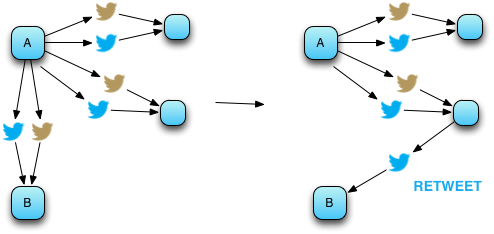
\includegraphics[scale=0.8]{6.Conclusions/Media/retweet_path.png} 
\caption{Using `filtered' edges to improve interestingness precision.}
\label{fig:removed_link}
\end{figure}

Therefore, the interestingness scores could be used to allow users to form conditional followships to other users, down which only interesting Tweets are sent. Figure \ref{fig:removed_link} initially shows user B receiving all of the Tweets from user A down a normal Twitter followship edge. However, if user B instead followed user A through a `filtered' edge, then only Tweets with a sufficient interestingness score would be received. Under this type of scheme, user B avoids receiving the uninteresting Tweets from A, thus increasing the chance of noticing the interesting ones.

%If this is the case, as with Figure \ref{fig:removed_link}, then the link representing the followship between the destination user (B) and the source user (A) could be unnecessary, since user B is receiving noise from user A, but the interesting information produced by user A could still reach B through retweets carried out by other followers of A. 

Of course, this system does require a set of users to be already following A in order to initially generate scores for each Tweet, but it does illustrate an interesting path for future research. Whilst largely hypothetical at this stage, it would provide an interesting extension to the research carried out in this thesis, in that interestingness scores could be used to assign thresholds of interestingness to users with the aim of discovering whether interesting Tweets could still be propagated to the extent that they deserve, yet by simultaneously reducing the propagation of noisy information. 

Since it has been explained how a user's followships act as a `search term' for information retrieval on Twitter, by finding ways of forwarding interesting information to users who do not directly (or `traditionally') follow a source, then it is clear how this could pave a way for enabling interesting and \textit{relevant} information can be delivered to users, yet without them having to look for it or know about its existence in the first place.


\section{Conclusions}
The work in this thesis was carried out with the aim of researching a methodology that is able to suitably infer interesting information in Twitter. Although the research has focused on Twitter as a platform for information dissemination, the motivation for this research stems from the \textit{noise} observed every day in all online social networks that support information propagation, including those such as Facebook and Tumblr.

The research processes culminated in the development of a method that ranks Tweets by assigning a score indicating an estimated level of interestingness based on a function of its perceived popularity. The methods were verified through the use of crowd-sourced validation tests covering the notions of general interestingness (in terms of identifying it from `noisy' information) and of more \textit{relevant} interestingness (through assessments of Tweets authored by more relevant users).

Analyses into the validation tests demonstrated the process by which users are able to identify interesting information and showed that the scoring mechanism is able to effectively rank Tweets in an appropriate order of interestingness in both mixed timelines and in timelines of Tweets authored by the same user. The scores can be applied to Tweets from all users on the same scale, meaning that inferences are not limited to a specific subset or type of Tweet.

The methods are open enough and use resources that are mostly common to many similar social networks. For example, ``shares'' and ``reblogs'' can be examined as the propagation mechanisms in Facebook and Tumblr, respectively, in attempts to apply the same scoring schemes to other platforms.


\section{Contributions}
Throughout the earlier chapters of this thesis, work has been conducted towards answering the hypothetical questions asked in Section \ref{section:research_questions} in the Introduction. The research has highlighted the inappropriateness of using retweet counts alone in indicating interestingness, and has shown the impact of the layout of users on the social graph on message propagation and how this can be useful for estimating Tweet interestingness. In particular, the questions are now answered more formally.

\textit{\textbf{RQ1} - Does Tweet popularity, measured in terms of retweets, \textbf{define} interesting (or non-`noisy') information?}\\
The number of retweets a particular Tweet receives cannot appropriately be used for defining interesting information. A Tweet that has been retweeted at least once is not necessarily interesting.

\textit{\textbf{RQ2} - Can Tweet popularity, measured in terms of retweets, \textbf{be an indicator} of interesting information?}\\
The number of retweets a Tweet has achieved is not alone indicative of its level of interestingness. The overall retweet count of a Tweet is produced as a function of its author's influence, and therefore Tweets written by different authors cannot have their Tweets' interestingness measured on the same scale.

\textit{\textbf{RQ3} - Is the arrangement of Twitter's social graph an important factor in retweet propagation, and thus perceived popularity?}\\
The layout of users and the edges connecting them on the social graph has been shown to strongly affect the permitted propagation of Tweets; some structures facilitate retweet spread, whilst others throttle it. The edge density also partially dictates users' influence levels, in that those users who are assigned a larger in-degree are more likely to achieve more retweets due to the magnitude of spread of the original Tweets. This importance was brought forward to the later work in identifying interesting Tweets.

\textit{\textbf{RQ4} - Can Tweet interestingness be inferred \textbf{non-semantically}?}\\
Chapter 5 showed that a Tweet's interestingness can be determined through a study of the Tweet's features and those of its author and the latter's relationship to others on the social graph. The inferences are therefore non-semantic, since they do not make any attempt to understand the content of individual words or phrases in the Tweets' contents. The method was also demonstrated to be suitable for ranking Tweets in order of interestingness \textit{level}, so that Tweets estimated to be more interesting could be shown at a higher priority.

As part of the research, several contributions to social media analytical research have been made, which have been discussed in the relevant chapters of the thesis and are summarised below. 

A comprehensive survey is carried out into relevant literature in information propagation in online social networks, along with evaluations and assessments of some of the research more specific to inferring interestingness.

Retweet properties and the way they are influenced by the social graph are thoroughly researched in order to provide a general background and understanding of the notions relating to propagation in online social networks, propagation and information penetration, Tweet `audience', and how these factors are related to the arrangement of users on the social graph. The definition of terms, such as `retweet group' and `maximum path-length' are useful for discussing various properties relating to retweeting on Twitter.

An investigative study is made into the use of machine learning techniques and classifiers in the field of social media, and the ways in which they can be useful for different purposes.

Finally, a numerical `definition' (or quantification) of estimated interestingness is contributed. A method for suitably predicting estimated retweet counts as dynamically nominal categories is described, implemented and verified, leading to the development of a method for assigning interestingness scores to Tweets as part of an effort to support the ranking of Tweets and of highlighting interesting Tweets from the noise of everyday communication on Twitter.


\chapter*{Appendices}
Source code, further diagrams, ideas, etc.


%%%%% BACK STUFF 
\backmatter

\def\baselinestretch{1.24}\normalfont

\bibliographystyle{plain}
\bibliography{includes/library}

\end{document}
